\chapter{Decoding Natural Scene Images from Mouse Visual Cortex}
\label{Chapter5} 

In the previous chapters, mice were probed with an abstract, temporally rich, stimulus presented as a stochastic sequence of visual visuals. In real-world environments, stimuli are enriched not only in temporal content, but spatial content. In this chapter, I take a different approach to investigate how categorical information is distributed in extrastriate areas using neurophysiology data and for a different kind of stimuli - natural scenes. Mice have multiple visual areas, as mentioned in Chapter \ref{Chapter1}, (Figure \ref{fig:vis_areas} and \ref{fig:retinomap}). These visual areas possess distinct brain-wide projection patterns \parencite{Wang2012} and also distinct spatiotemporal response properties to grating stimuli  \parencite{Andermann2011,Marshel2011,Roth2012,Glickfeld2013a,Tohmi2014,Juavinett2015}. However, little is known as to whether mouse secondary visual areas also specialize in processing natural scene images. The goal of this chapter is to test whether the identity or category of natural scene images can be decoded from the neural population activity of distinct higher visual areas in the mouse.\par 

The brain, ultimately, uses information in complex scenes to recognize salient stimuli, discriminate amongst objects in a scene, and make decisions. Hierarchical visual processing is a hallmark of object recognition observed in the primate ventral stream pathway \parencite{DiCarlo2012}. To illustrate with an example, imagine you are faced with a task to discern between a car and a horse crossing the street. The information needed to make the categorization is already available at the level of the retina, however the information lives in a tangled and conflated representation. As the information progresses through various stages of visual processing along the ventral steam, the representations becomes more untangled, i.e. more linearly separable. Ultimately the distinction between the horse and the car are easily distinguishable and linearly separable in neural activity space. At the highest stage of visual processing, a linear boundary can be drawn between the neuronal population representation between the horse and the car. Linear readout (i.e. linear combinations) of neurons is an assumption for how downstream (postsynaptic) brain areas might theoretically integrate information represented in the neural responses of upstream (presynaptic) brain areas to ultimately generate an action.  

Population decoding analysis has been a fruitful tool for studying this type of high-level visual processing and revealing information represented within a neural population \parencite{Hung2005,Rust2010a,Pagan2013}. Population decoders (or classifiers) address questions such as, given neural population activity in a brain area, can information be read out about external variables in the world (eg. stimulus, choice)? In this chapter, I ask the following questions: how linearly separable are the neural responses to natural scenes? How does linear separability change across multiple visual areas and across cortical layers within an area? In other words, can a linear decoder read out the natural scene identity (or category) given the neural activity patterns in a given visual brain area or cortical layer? Since natural scenes are collection of objects, I drew inspiration from object recognition processing in primate ventral stream in considering how to address the proposed questions.  

To do this, I compared how natural scenes are processed in multiple mouse visual areas and cortical layers. More precisely I tested whether the neural population activity in response to distinct natural scenes was linearly separable. To this end, I trained a classifier to decoded the identity (or category) of natural scene images presented to mice, and compared the decoder accuracy across multiple visual areas and layers. The hypothesis is that activity in higher visual areas in response to natural scenes are linearly separable, consistent with an 'untangled' neural representation along the visual processing hierarchy. 

%-----------------------------------------------------------------------------
\begin{figure}
  \centering
   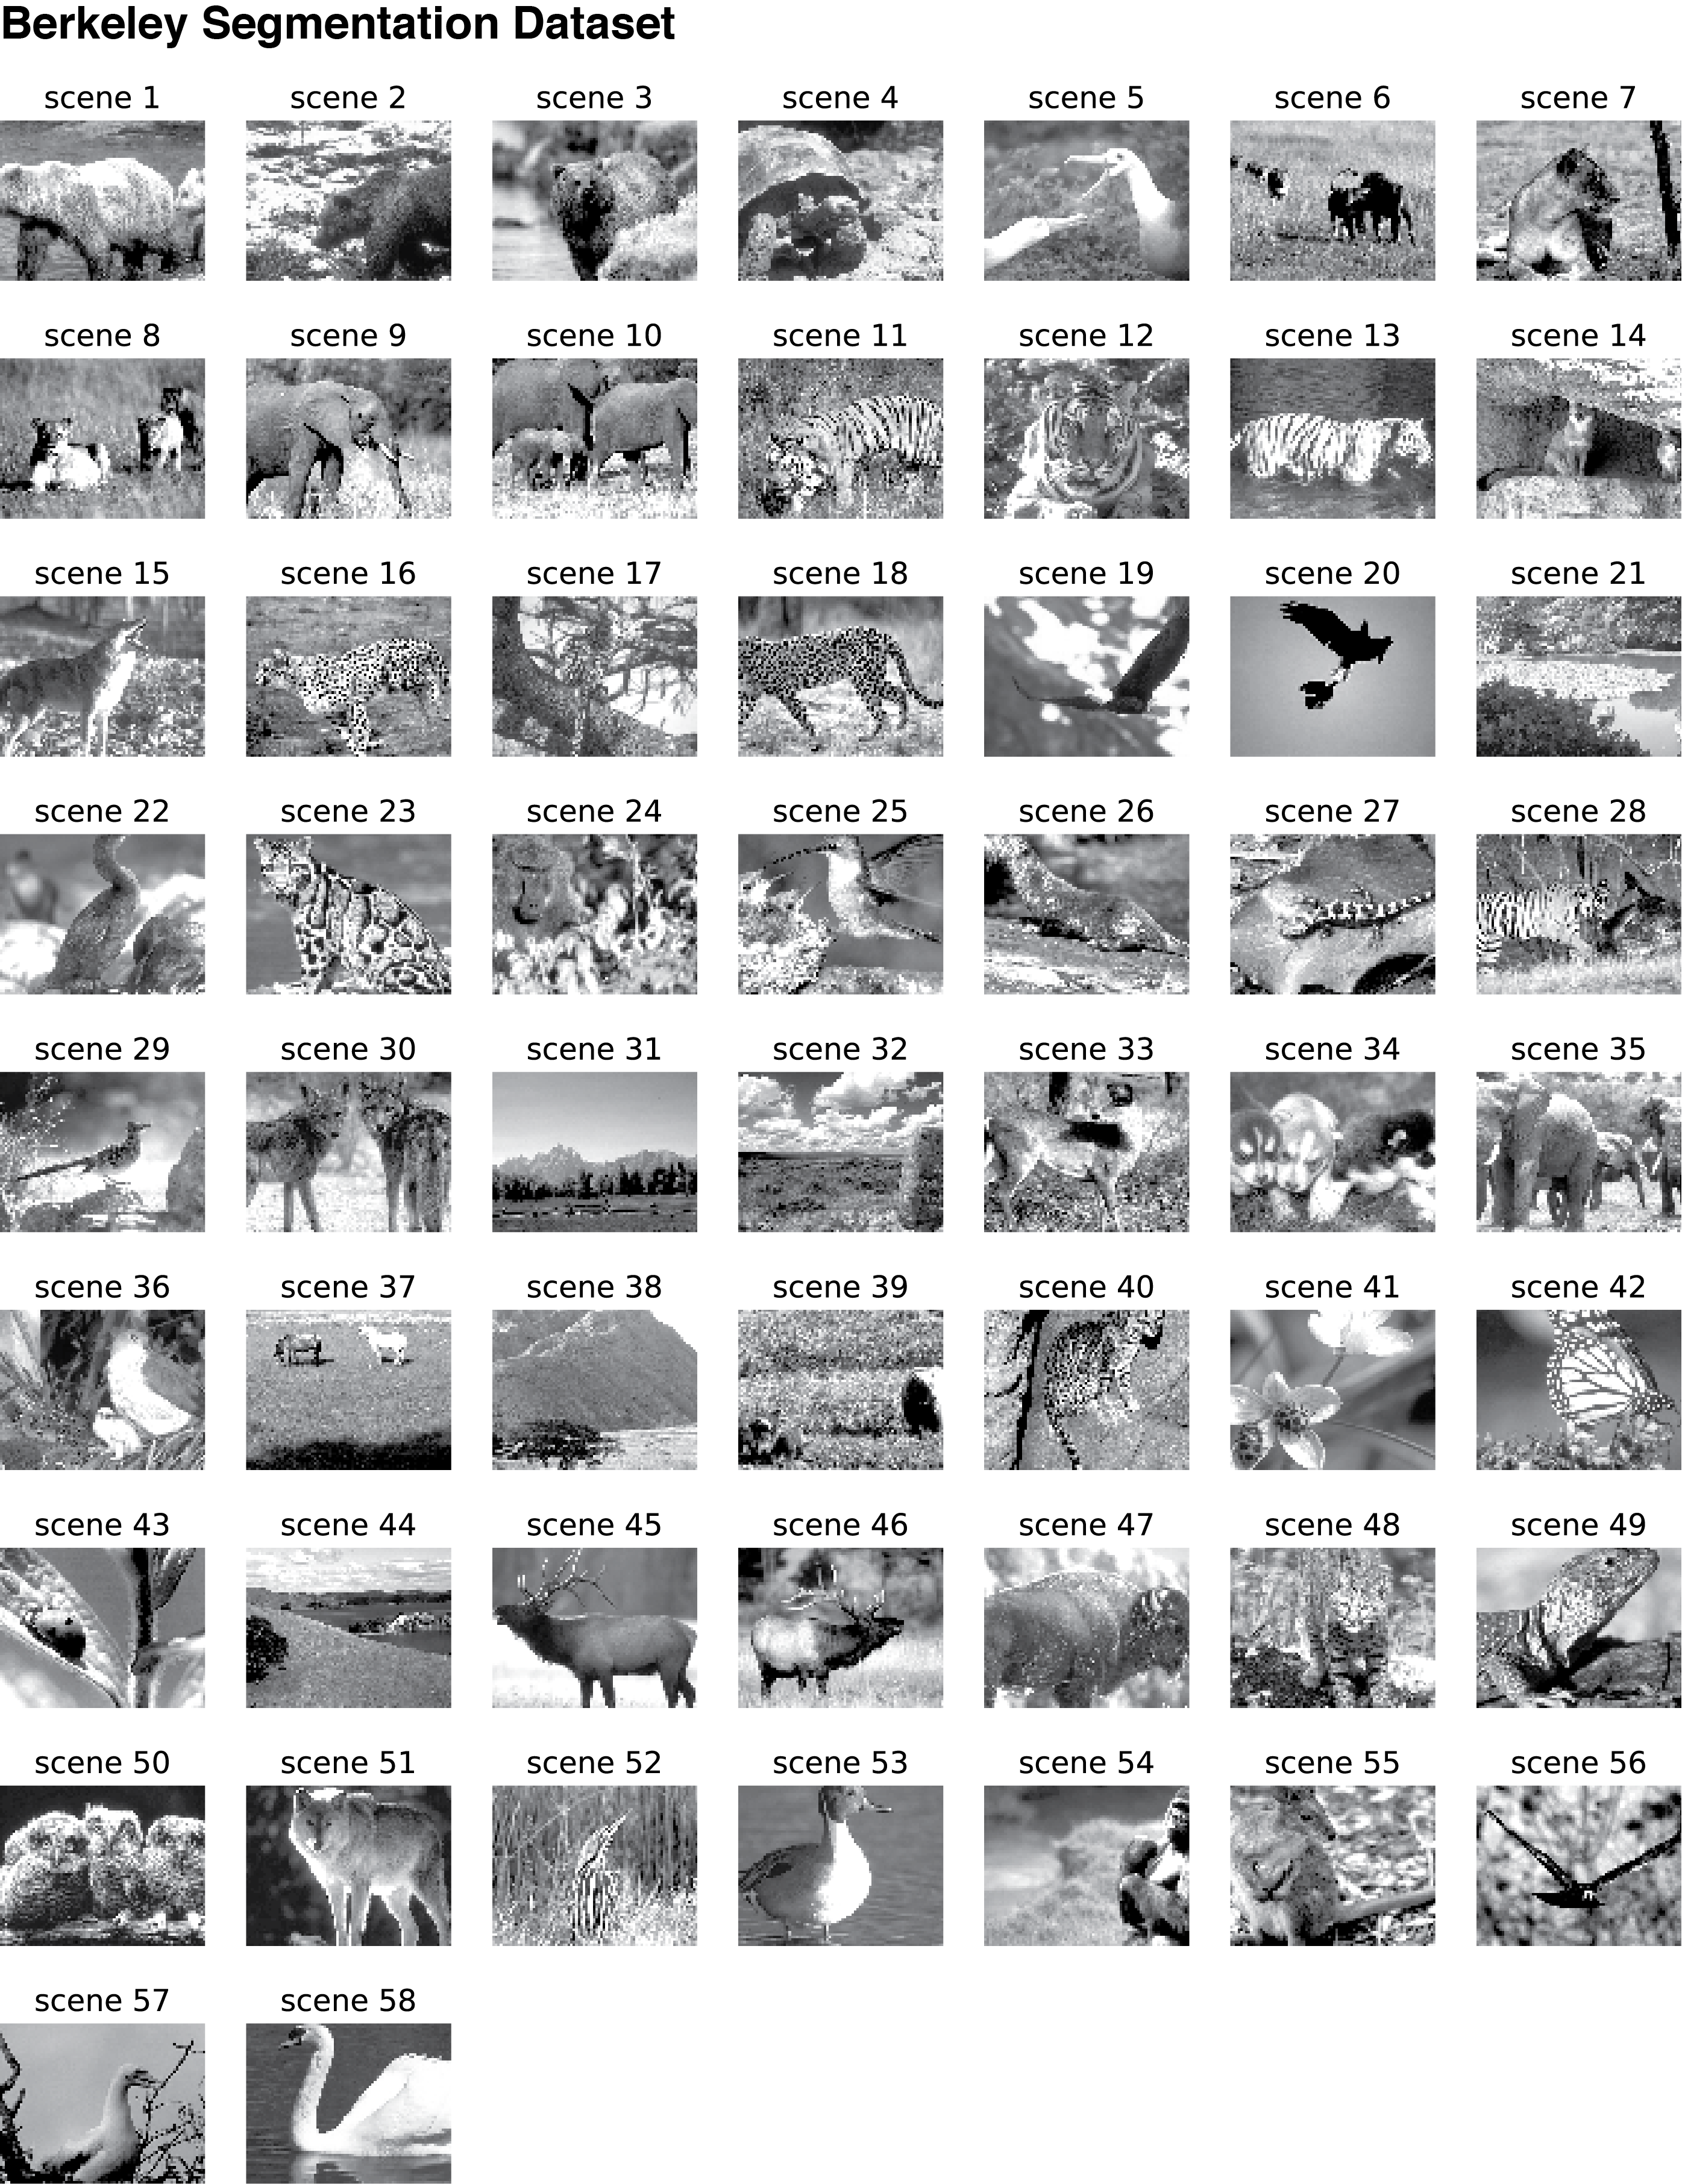
\includegraphics[width=\textwidth,height=0.9\textheight,keepaspectratio]{Figures/chapter5/images_dataset1.png}
  \caption[Thumbnail of Natural Images Stimulus Set - Part 1]{\textbf{Thumbnail of Natural Images Stimulus Set - Part 1} }
   \label{fig:images1}
\end{figure}
%-----------------------------------------------------------------------------
\begin{figure}
  \centering
   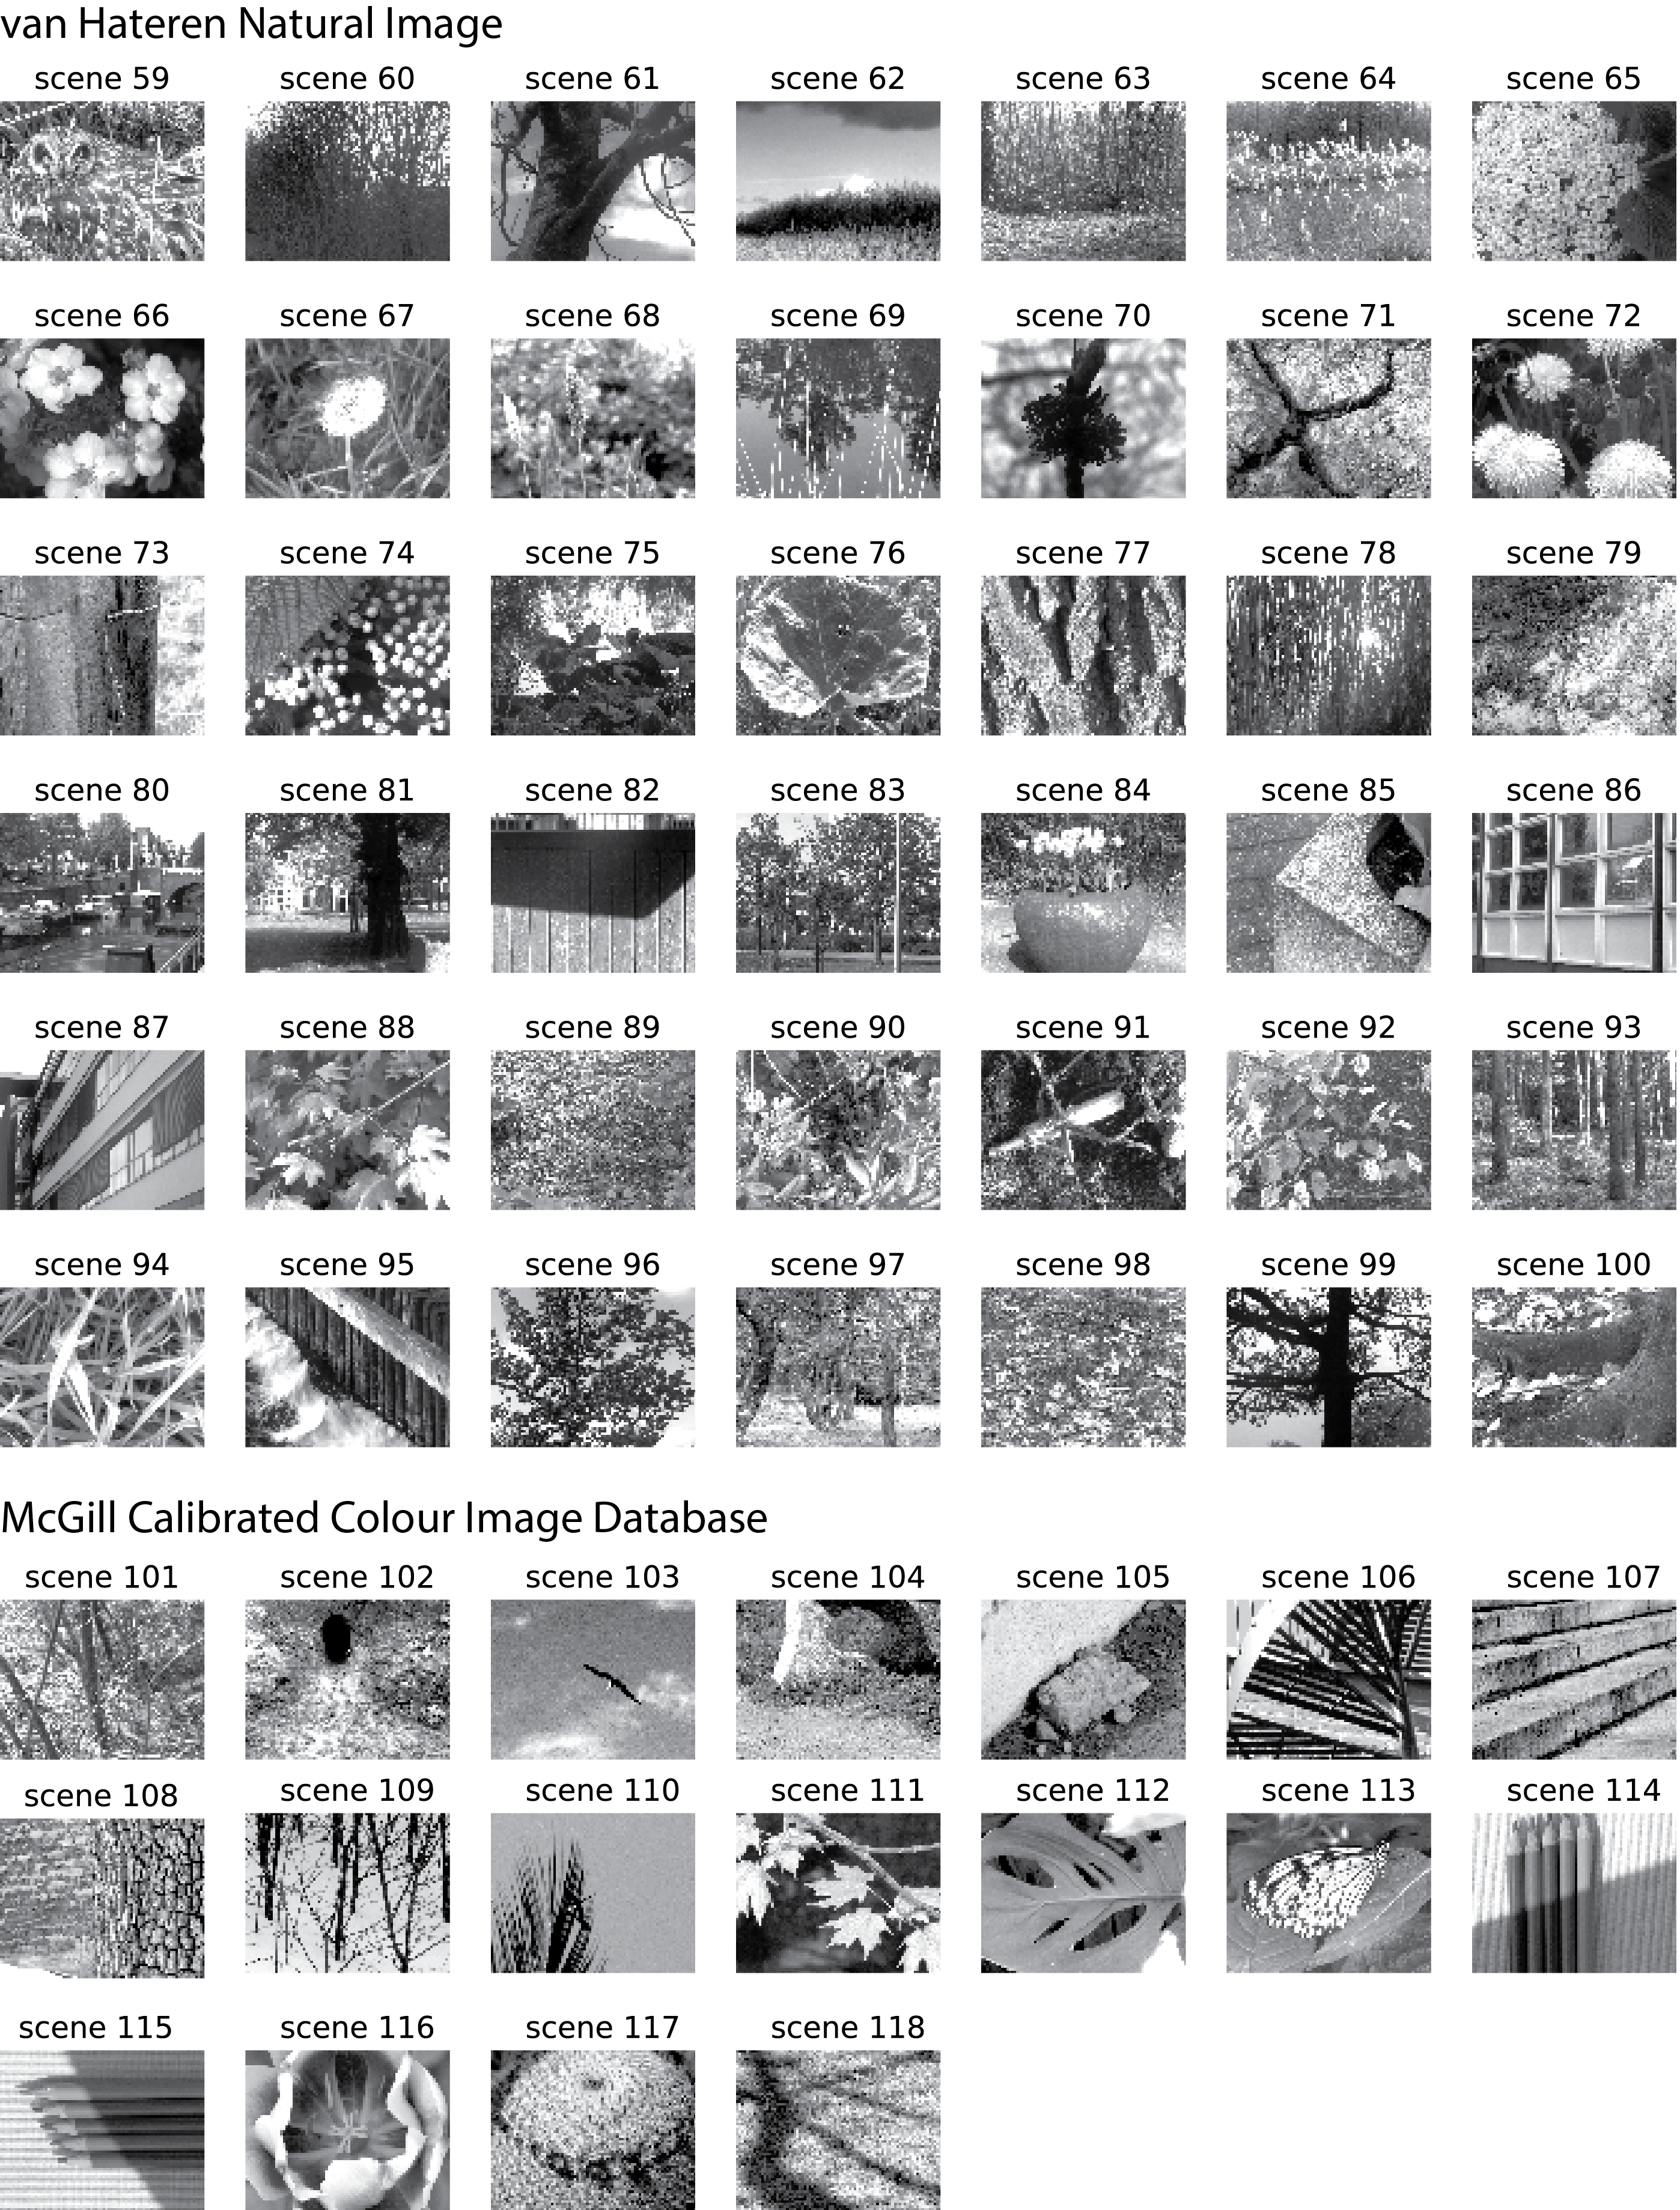
\includegraphics[width=\textwidth,height=0.9\textheight,keepaspectratio]{Figures/chapter5/images_dataset2.png}
  \caption[Thumbnail of Natural Images Stimulus Set - Part 2]{\textbf{Thumbnail of Natural Images Stimulus Set - Part 2} }
   \label{fig:images2}
\end{figure}
%-----------------------------------------------------------------------------
\section{Data and Methods for Analysis}
The dataset used for the analyses in this chapter was obtained from the Allen Brain Observatory public dataset (\url{http://observatory.brain-map.org/visualcoding/} and \textcite{Hawrylycz2016}). The dataset consists of neural responses from over 27,000 cells across four secondary visual areas and multiple cortical layers. Neural responses were recorded from mice passively viewing numerous visual stimuli, including static and drifting gratings, sparse noise, natural scenes, and natural movies. In particular, I analyzed data from the natural scenes sessions. 

Mice were presented with a total of 118 natural scenes (Figures \ref{fig:images1} and \ref{fig:images2}). Full screen images (1174 x 918 pixels) were presented in gray scale, matched for luminance, and contrast normalized. The images were obtained from public image databases: Berkeley Segmentation Dataset \parencite{Martin2001}, van Hateren Natural Image Dataset \parencite{VanHateren1998}, and the McGill Calibrated Colour Image Database \parencite{Olmos2004}. Each scene was presented for 250 ms and repeated 50 times, randomly. The images were presented consecutively, without an inter-stimulus interval. A blank screen was presented after ever 100 scenes. 

For each visual area, the data was organized into a matrix \emph{XT}, of size \emph{n} x \emph{c} x \emph{t}, where n = number of trials, c = number of cells in a visual area (or cell type), and t = time (or imaging frames).  Each cell had a total of 5900 trials (118 images, 50 repeats each). Blank stimulus trials were excluded in the analysis. The number of cells per area ranged between 2157 (area PM) to 4189 (V1) (Table \ref{celltable}). The data was acquired at approximately 31 frames per second and thus approximately 7 imaging frames were acquired per 250ms of stimulus presentation. Included in \emph{XT} was the pre-stimulus and post-stimulus response, each 250 ms in length. The analyses in this project were done using the relative changes in fluorescence ($\Delta$ F/F) as the neuronal response rather than inferred spike events.
%-----------------------------------------------------------------------------
%-----------------------------------------------------------------------------
\begin{table}
\centering
\begin{tabular}{@{}ccccc@{}}
\toprule
\begin{tabular}[c]{@{}c@{}}Layers\\ (Cre line)\end{tabular} & PM   & AL   & LM   & V1   \\ \midrule
\begin{tabular}[c]{@{}c@{}}2/3\\ (Cux-cre)\end{tabular}    & 1646 & 1380 & 1580 & 2802 \\
\begin{tabular}[c]{@{}c@{}}4\\ (Rorb-cre)\end{tabular}     & 208  & 480  & 530  & 821  \\
\begin{tabular}[c]{@{}c@{}}5\\ (Rbp4-cre)\end{tabular}     & 303  & 463  & 496  & 566  \\ \bottomrule
\begin{tabular}[c]{@{}c@{}}Total cells\end{tabular}        & 2157  & 2323  & 2606  & 4189  \\
\end{tabular}
\caption{Cells per Layer per Visual Area}
\label{celltable}
\end{table}
%-----------------------------------------------------------------------------
%-----------------------------------------------------------------------------

To measure performance on identifying natural scenes given a neural activity pattern, I trained a linear support vector classifier (SVM, one-vs-rest classifier scheme) on the average response during 200-300ms post stimulus onset, and computed cross-validated test accuracy for the trained classifier for each area. The classifier was trained on 70\% of the trials in an area, and tested on the remaining 30\%. In most cases I repeated this procedure 10 times to obtain an average and standard error of the mean (SEM). The SVM linear classifier procedure is similar to the approach used in previous studies in primate visual object recognition \parencite{Hung2005,Rust2010a}
%-----------------------------------------------------------------------------
%-----------------------------------------------------------------------------
\section{Results}
\subsection{Decoding Natural Scene Identity}
The first task was to decode the identity of natural scenes given the population activity from each area. All the visual areas performed well above chance level (0.85\%) on the identity task (Figure \ref{fig:decodebar} a). Primary visual cortex (V1) exhibited the highest performance (>75\%) on linearly classifying the natural images, followed by area LM (>50\%). Area LM is an anatomical equivalent of primate V2 because it is the most prominent recipient of V1 projections and LM projects to all visual areas \parencite{Wang2012}. LM and AL have also been referred to as the gateways into the putative mouse ventral and dorsal processing streams based on evidence from cytoarchitecture and anatomical projections \parencite{wang2011,Wang2013a}.  Areas AL and PM performed similarly (> 30\%). To make sure that the performance accuracy of V1 was not merely due to uneven total number of neurons across visual areas, I repeated the decoding image identity task with 2100 neurons from each areas. As shown in Figure \ref{fig:decodebar}b, the trend in performance accuracy across areas remains; however the overall accuracy is decreased for each area. This is consistent with the observation that performance accuracy increases with the size of the population for each area (Figure \ref{fig:decodepop}).\par 
%-----------------------------------------------------------------------------
\begin{figure}
  \centering
    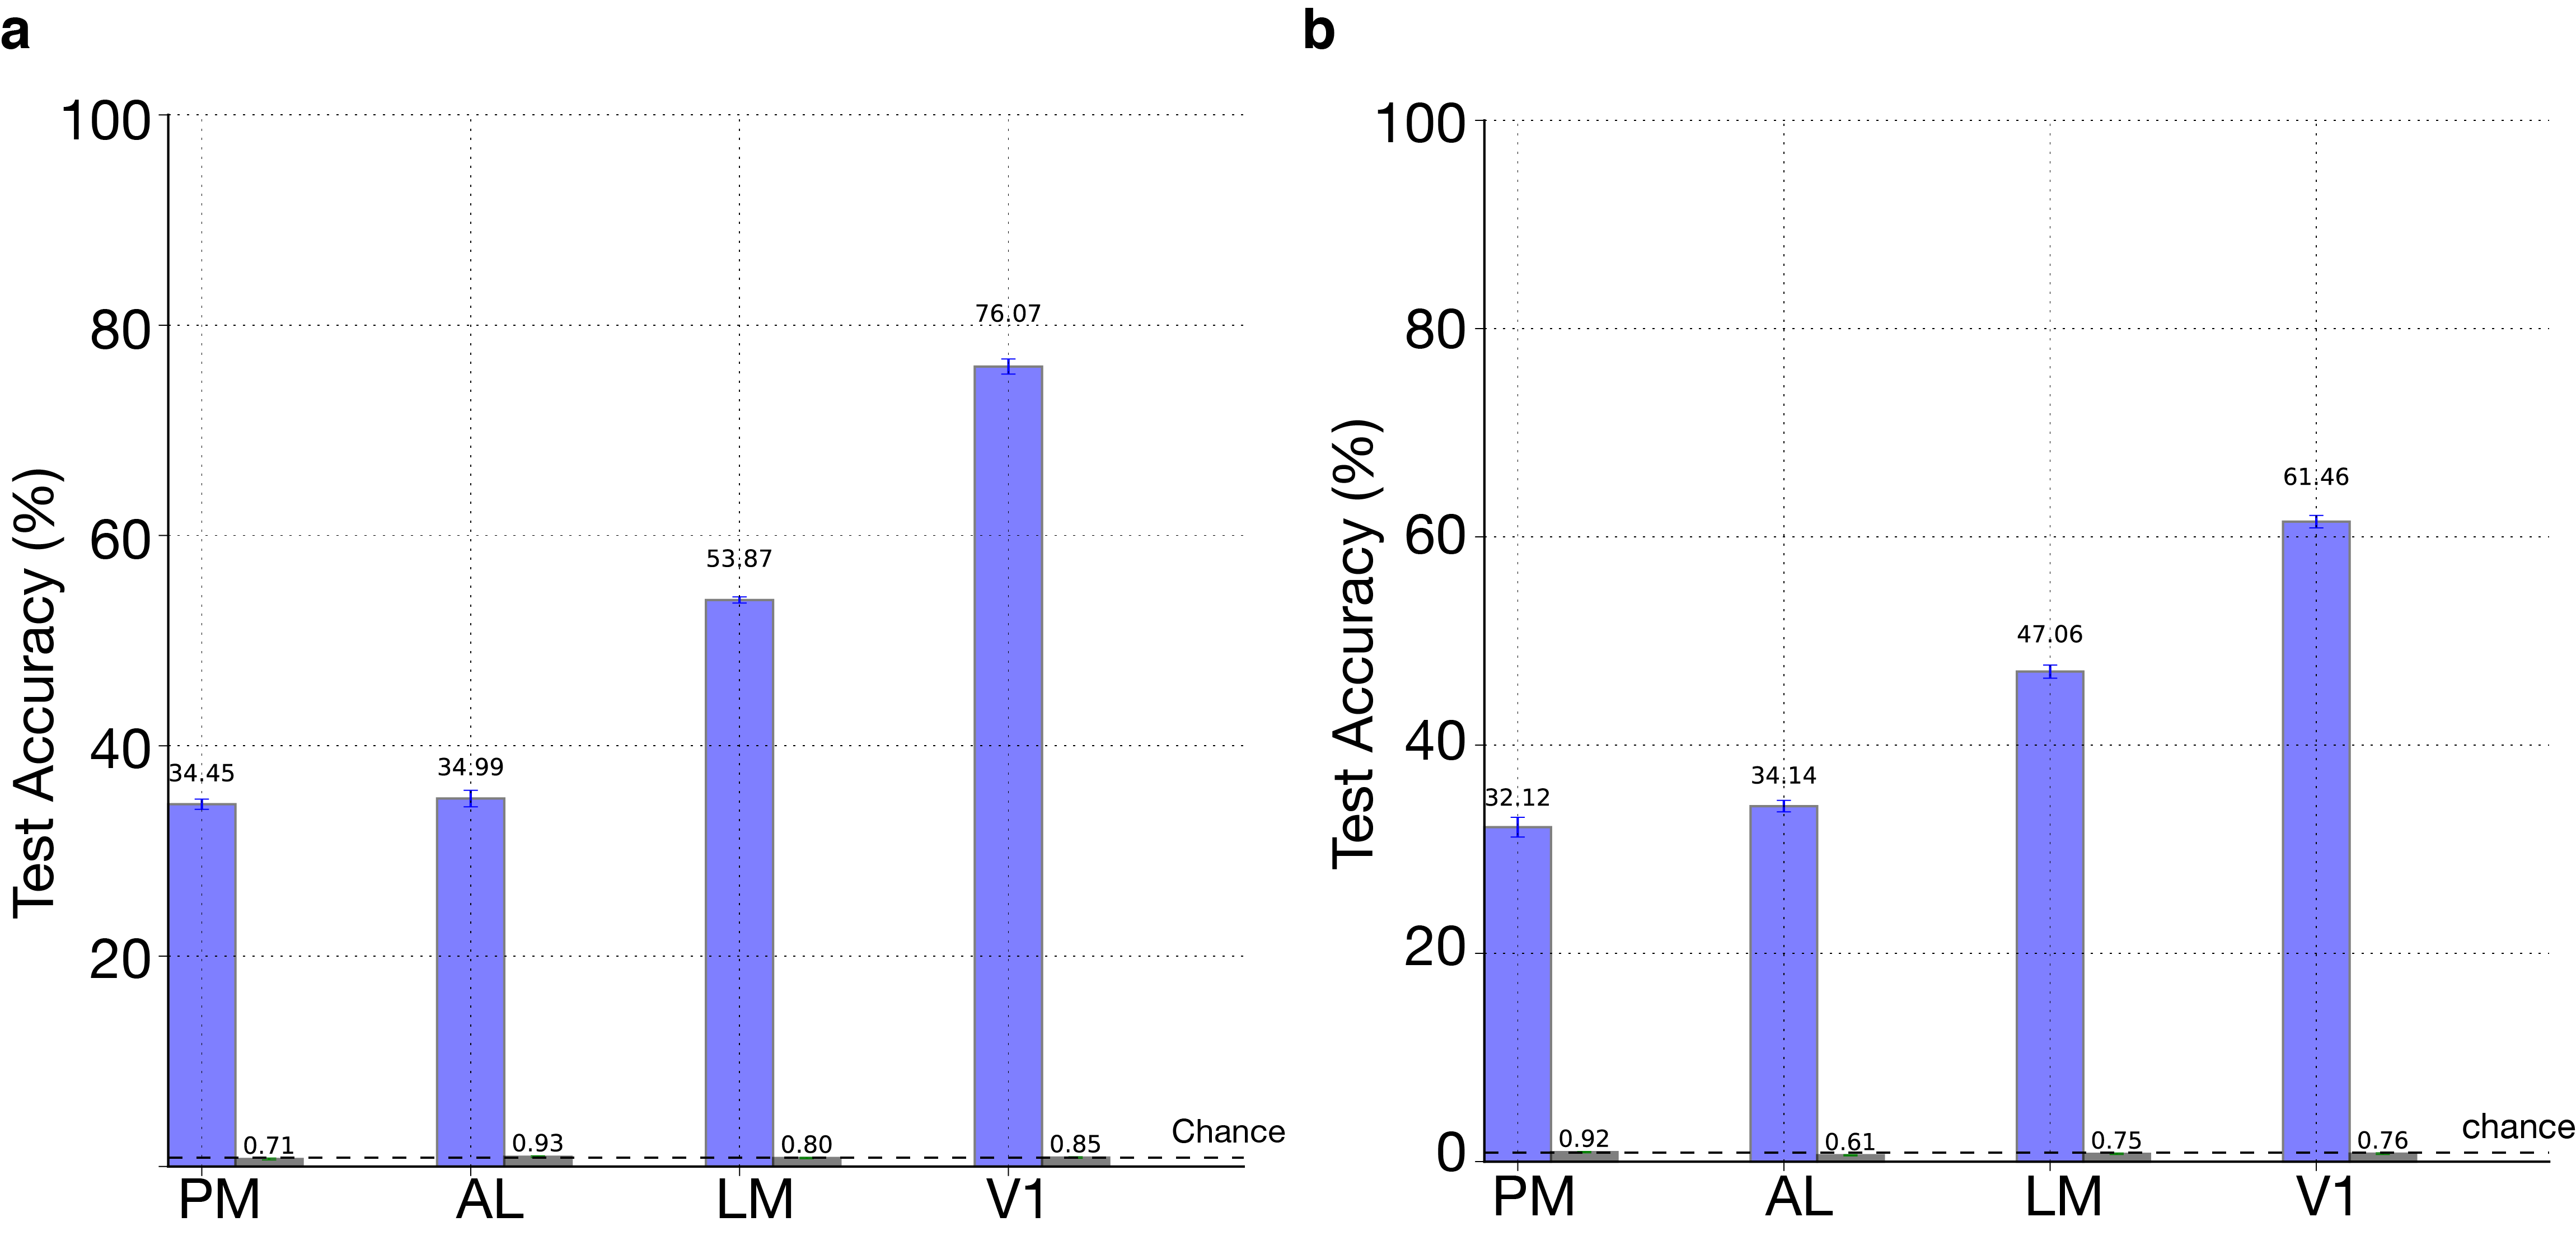
\includegraphics[width=\textwidth]{Figures/chapter5/accuracy_all_and_2100_neurons.png}
%   	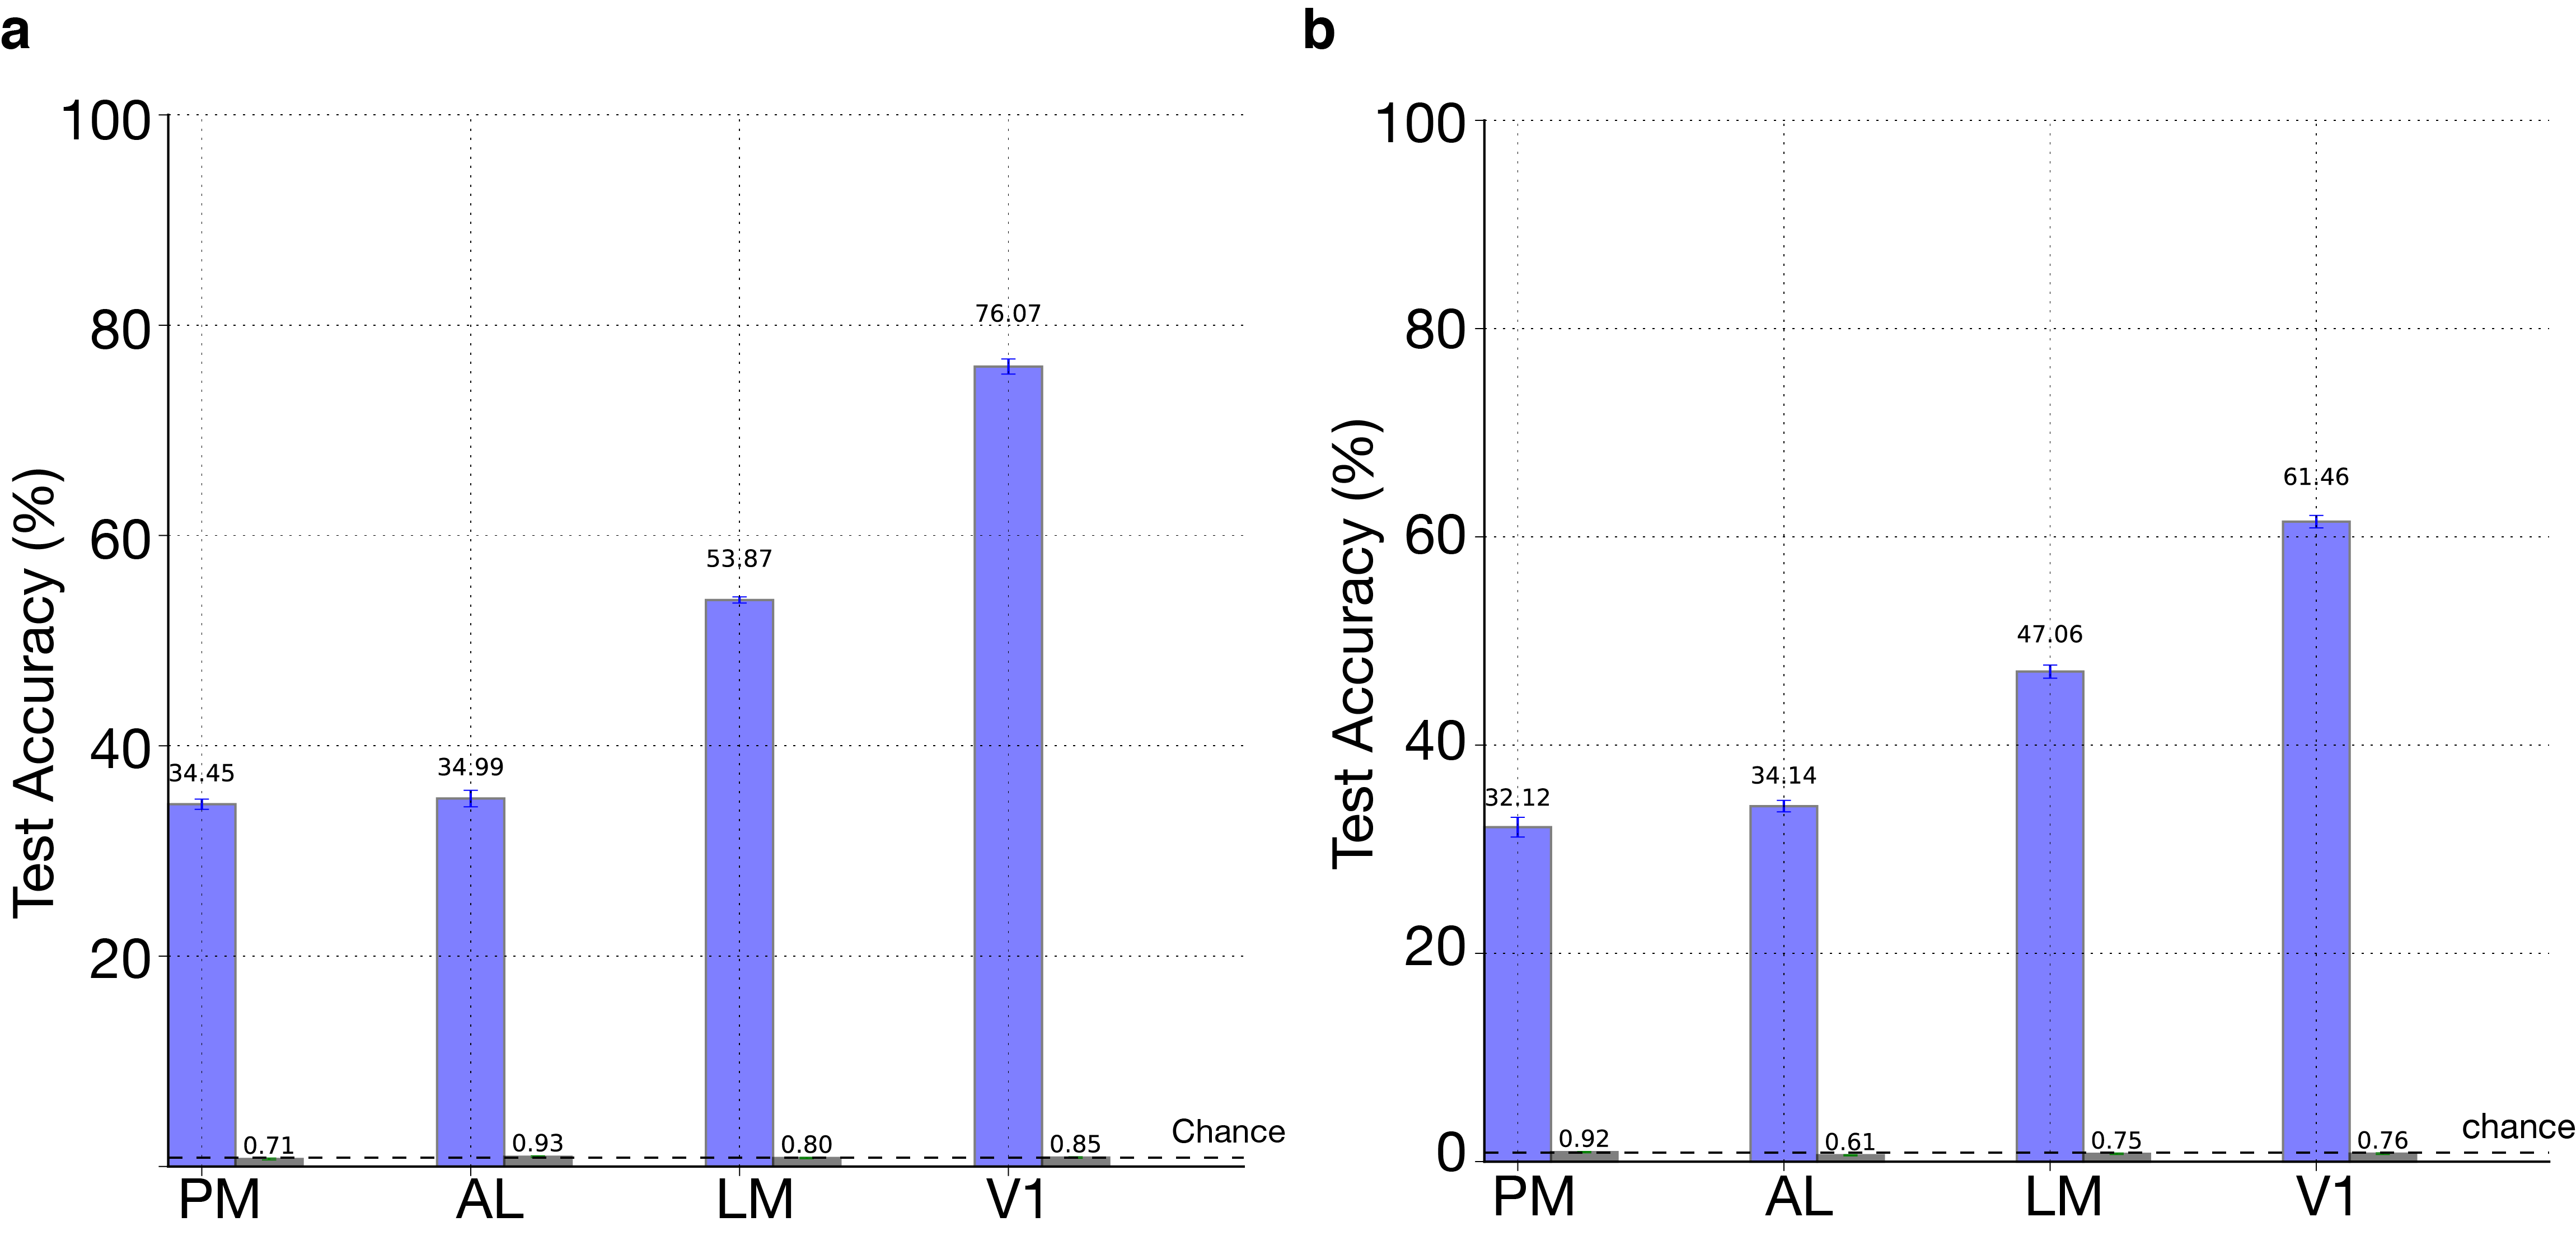
\includegraphics[scale=0.35]{Figures/chapter5/accuracy_all_and_2100_neurons.png}
    \caption[Decoder Test Accuracy]{\textbf{Decoder Test Accuracy} (a) including all neurons per visual area and (b) including a subset of 2100 neurons per visual area. Purple bars represent decoder test accuracy. Gray bars represent shuffled label controls. Error bars represent standard error of the mean.}
  \label{fig:decodebar}
\end{figure}
%-----------------------------------------------------------------------------
\begin{figure}
  \centering
    	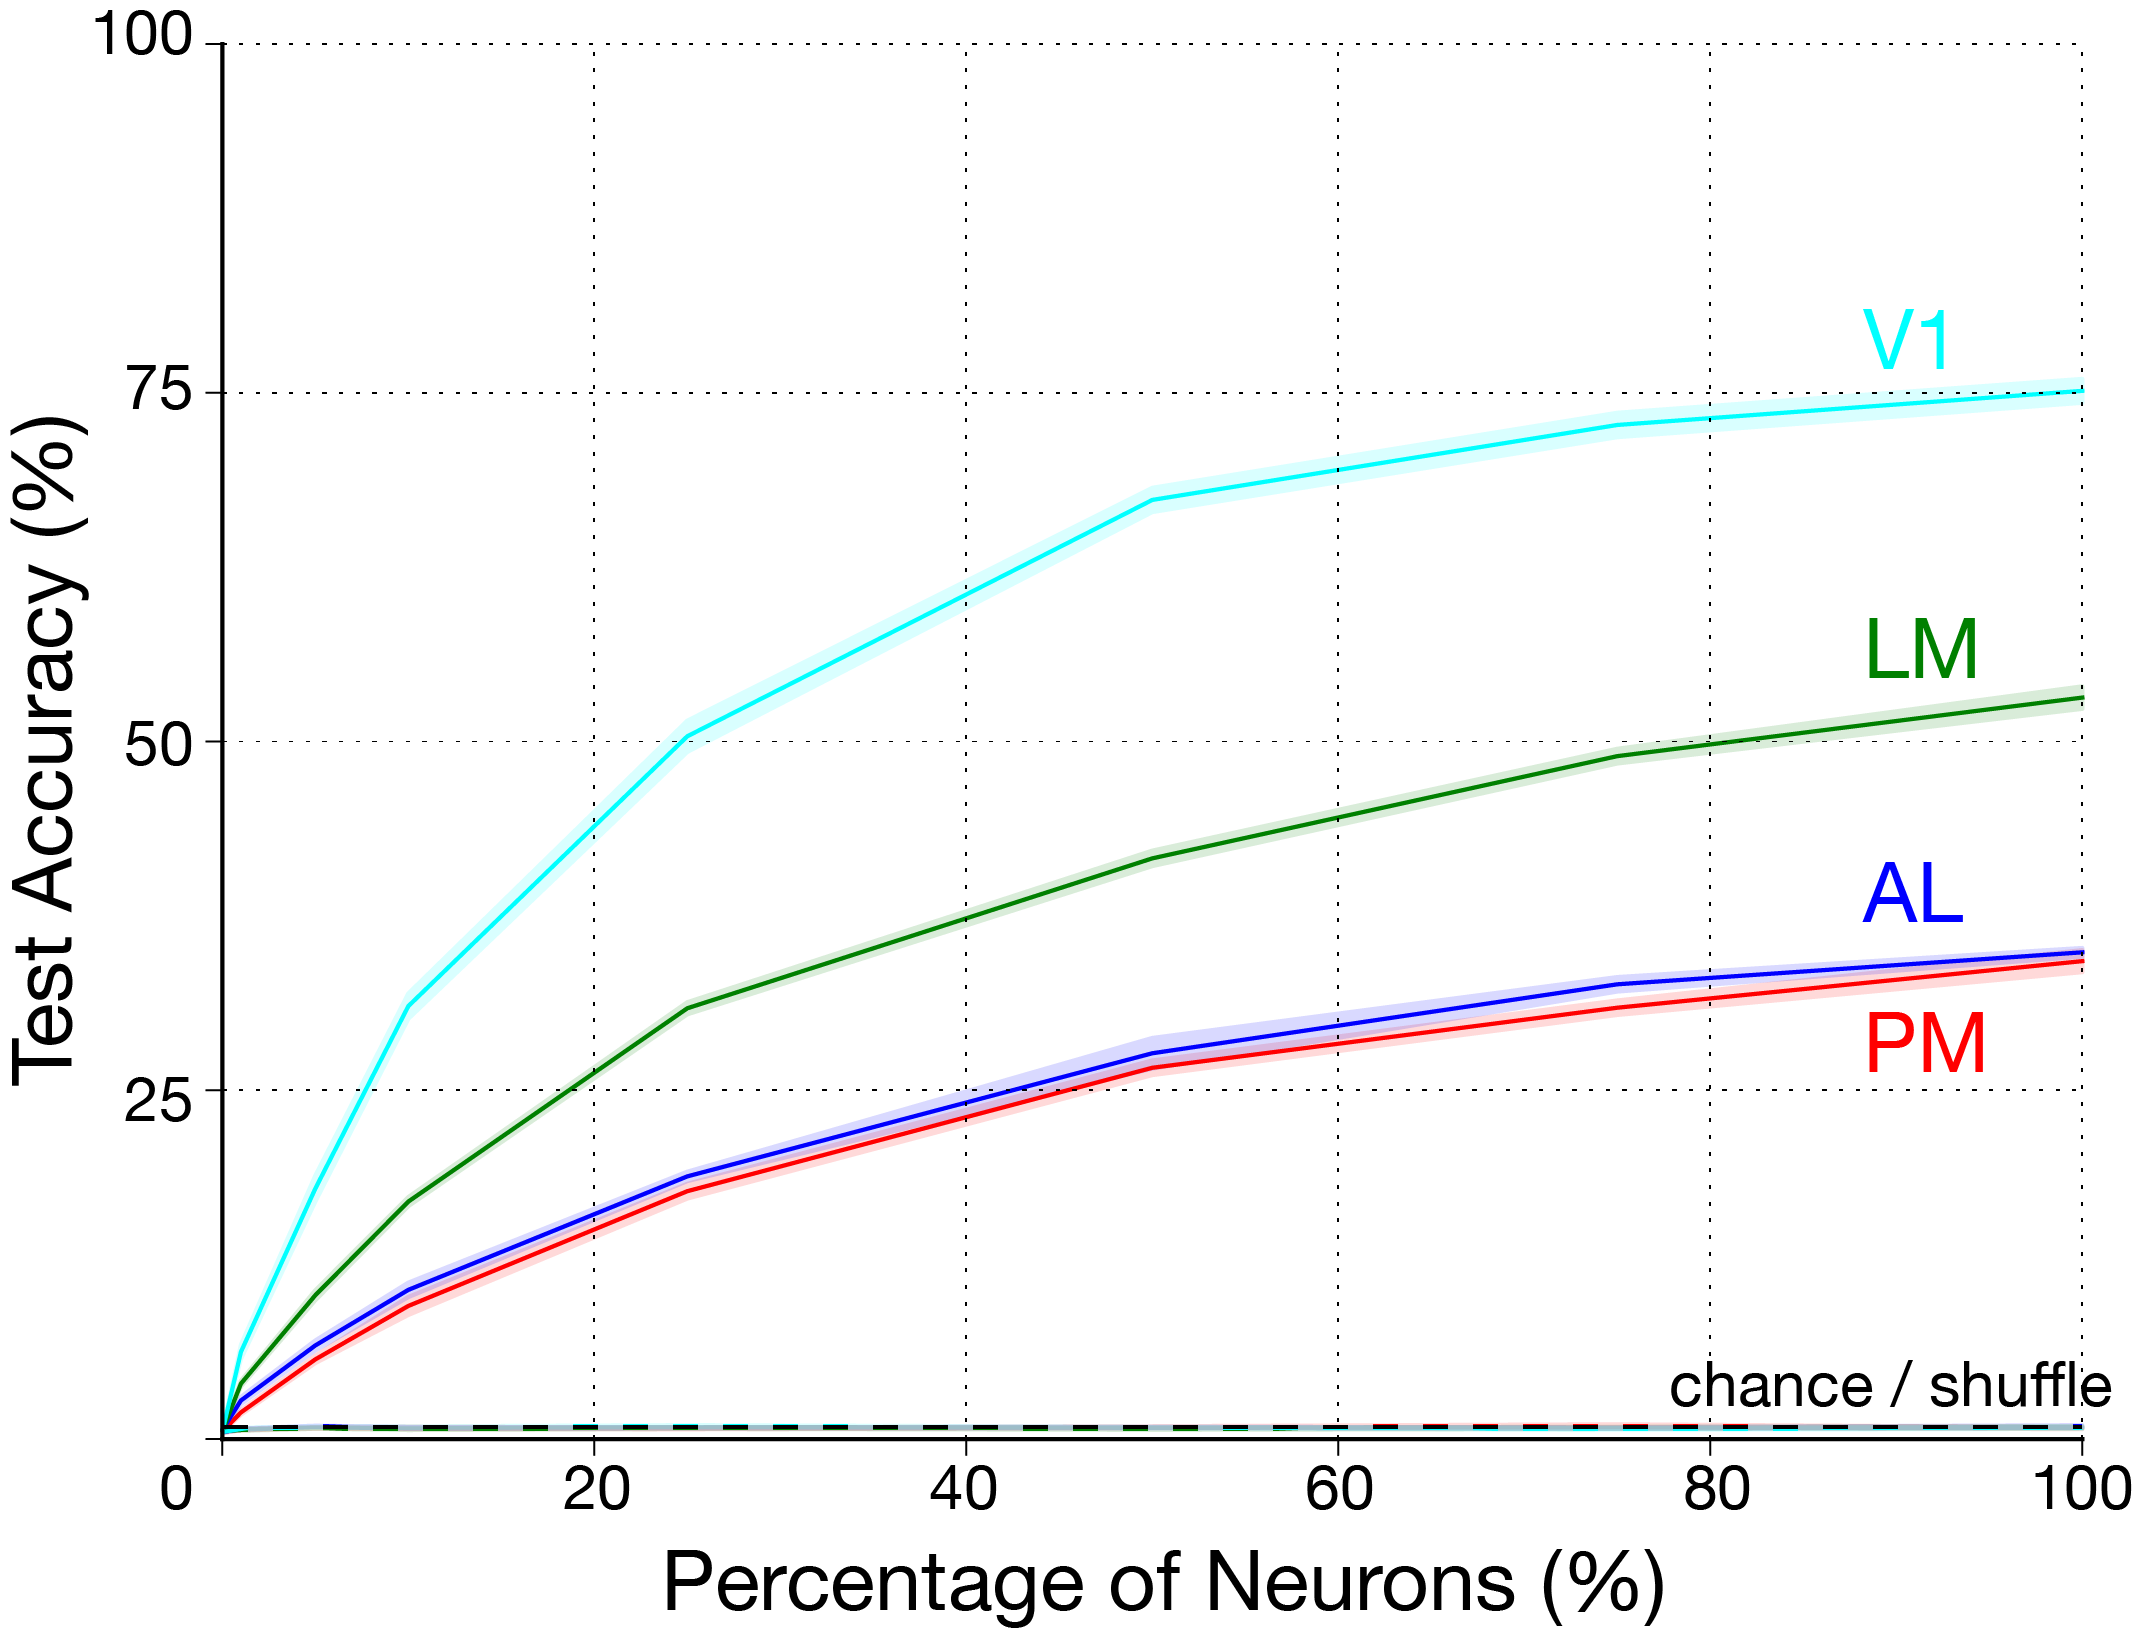
\includegraphics[width=\textwidth]{Figures/chapter5/accuracy_population.png}
%   	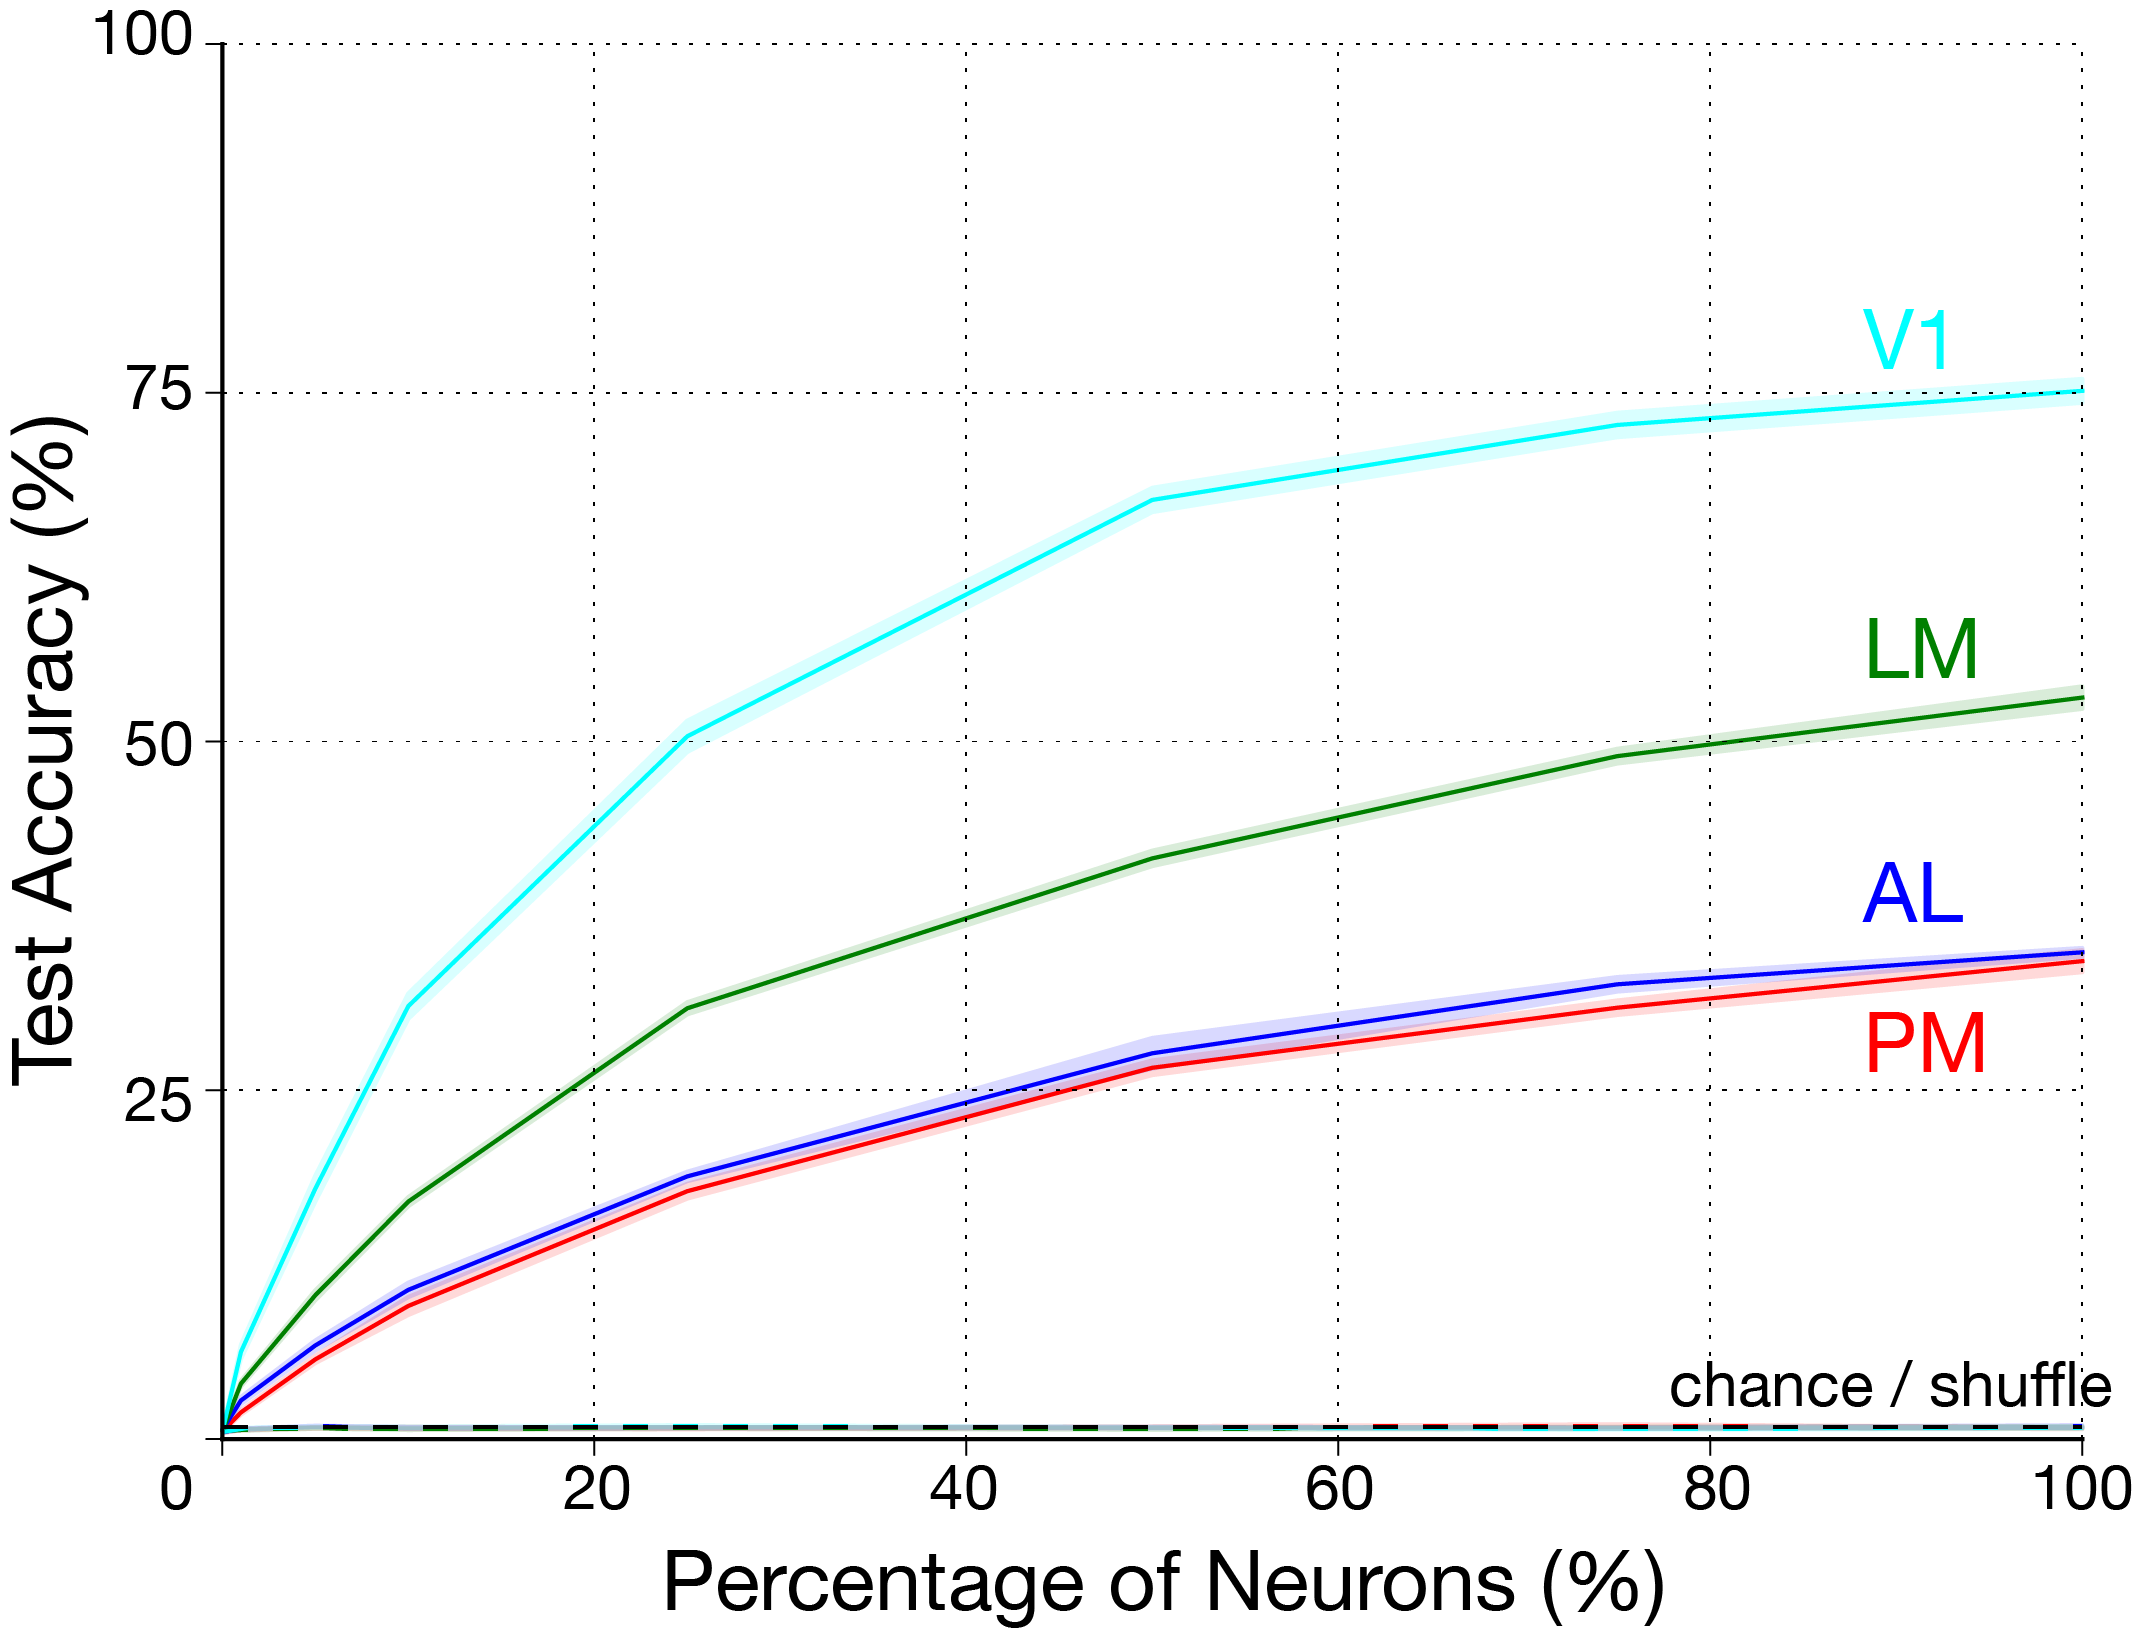
\includegraphics[scale=0.45]{Figures/chapter5/accuracy_population.png}
    \caption[Decoder Accuracy Per Visual Area Population Size]{\textbf{Decoder Accuracy Per Visual Area Population Size}. Test accuracy increases with number of neurons for each visual area. Solid line represents test accuracy. Shaded error bars represent standard error of the mean.}
  \label{fig:decodepop}
\end{figure}
%-----------------------------------------------------------------------------
To evaluate and compare each classifier’s performance, I created a confusion matrix (Figure \ref{fig:confusion}), which compares the classifier’s predicted image identity label and the true image label. The confusion matrix shows the proportion of cases the classifier predicted the true image label, otherwise known as the conditional probability (\emph{P(predicted|true)}) of the classifier predicted label given the true label. The confusion matrix also shows which images elicit similar neural population responses. From the confusion matrix, I computed the mutual information (\emph{MI}) between the classifier's prediction and the true image label: 
\begin{equation}
\begin{aligned}
MI = \sum_{l} \sum_{l'} P(l',l) log_2 \frac{P(l',l)}{P(l')P(l)} \\
P(l) = \sum_{l} P(l',l) \\
P(l') = \sum_{l'} P(l',l)
\end{aligned}
\label{eq:mutualinfo}
\end{equation}
Where \emph{l} is the true image label, \emph{l'} is the predicted image label, \emph{P(l',l)} is the joint probability (normalized confusion matrix), \emph{P(l)} and \emph{P(l')} are the marginal probability distributions. Similar to the identity decode performance accuracy, the mutual information increases with the size of the population (Figure \ref{fig:mutualinfopop}).\par 
%-----------------------------------------------------------------------------
\begin{figure}
  \centering
     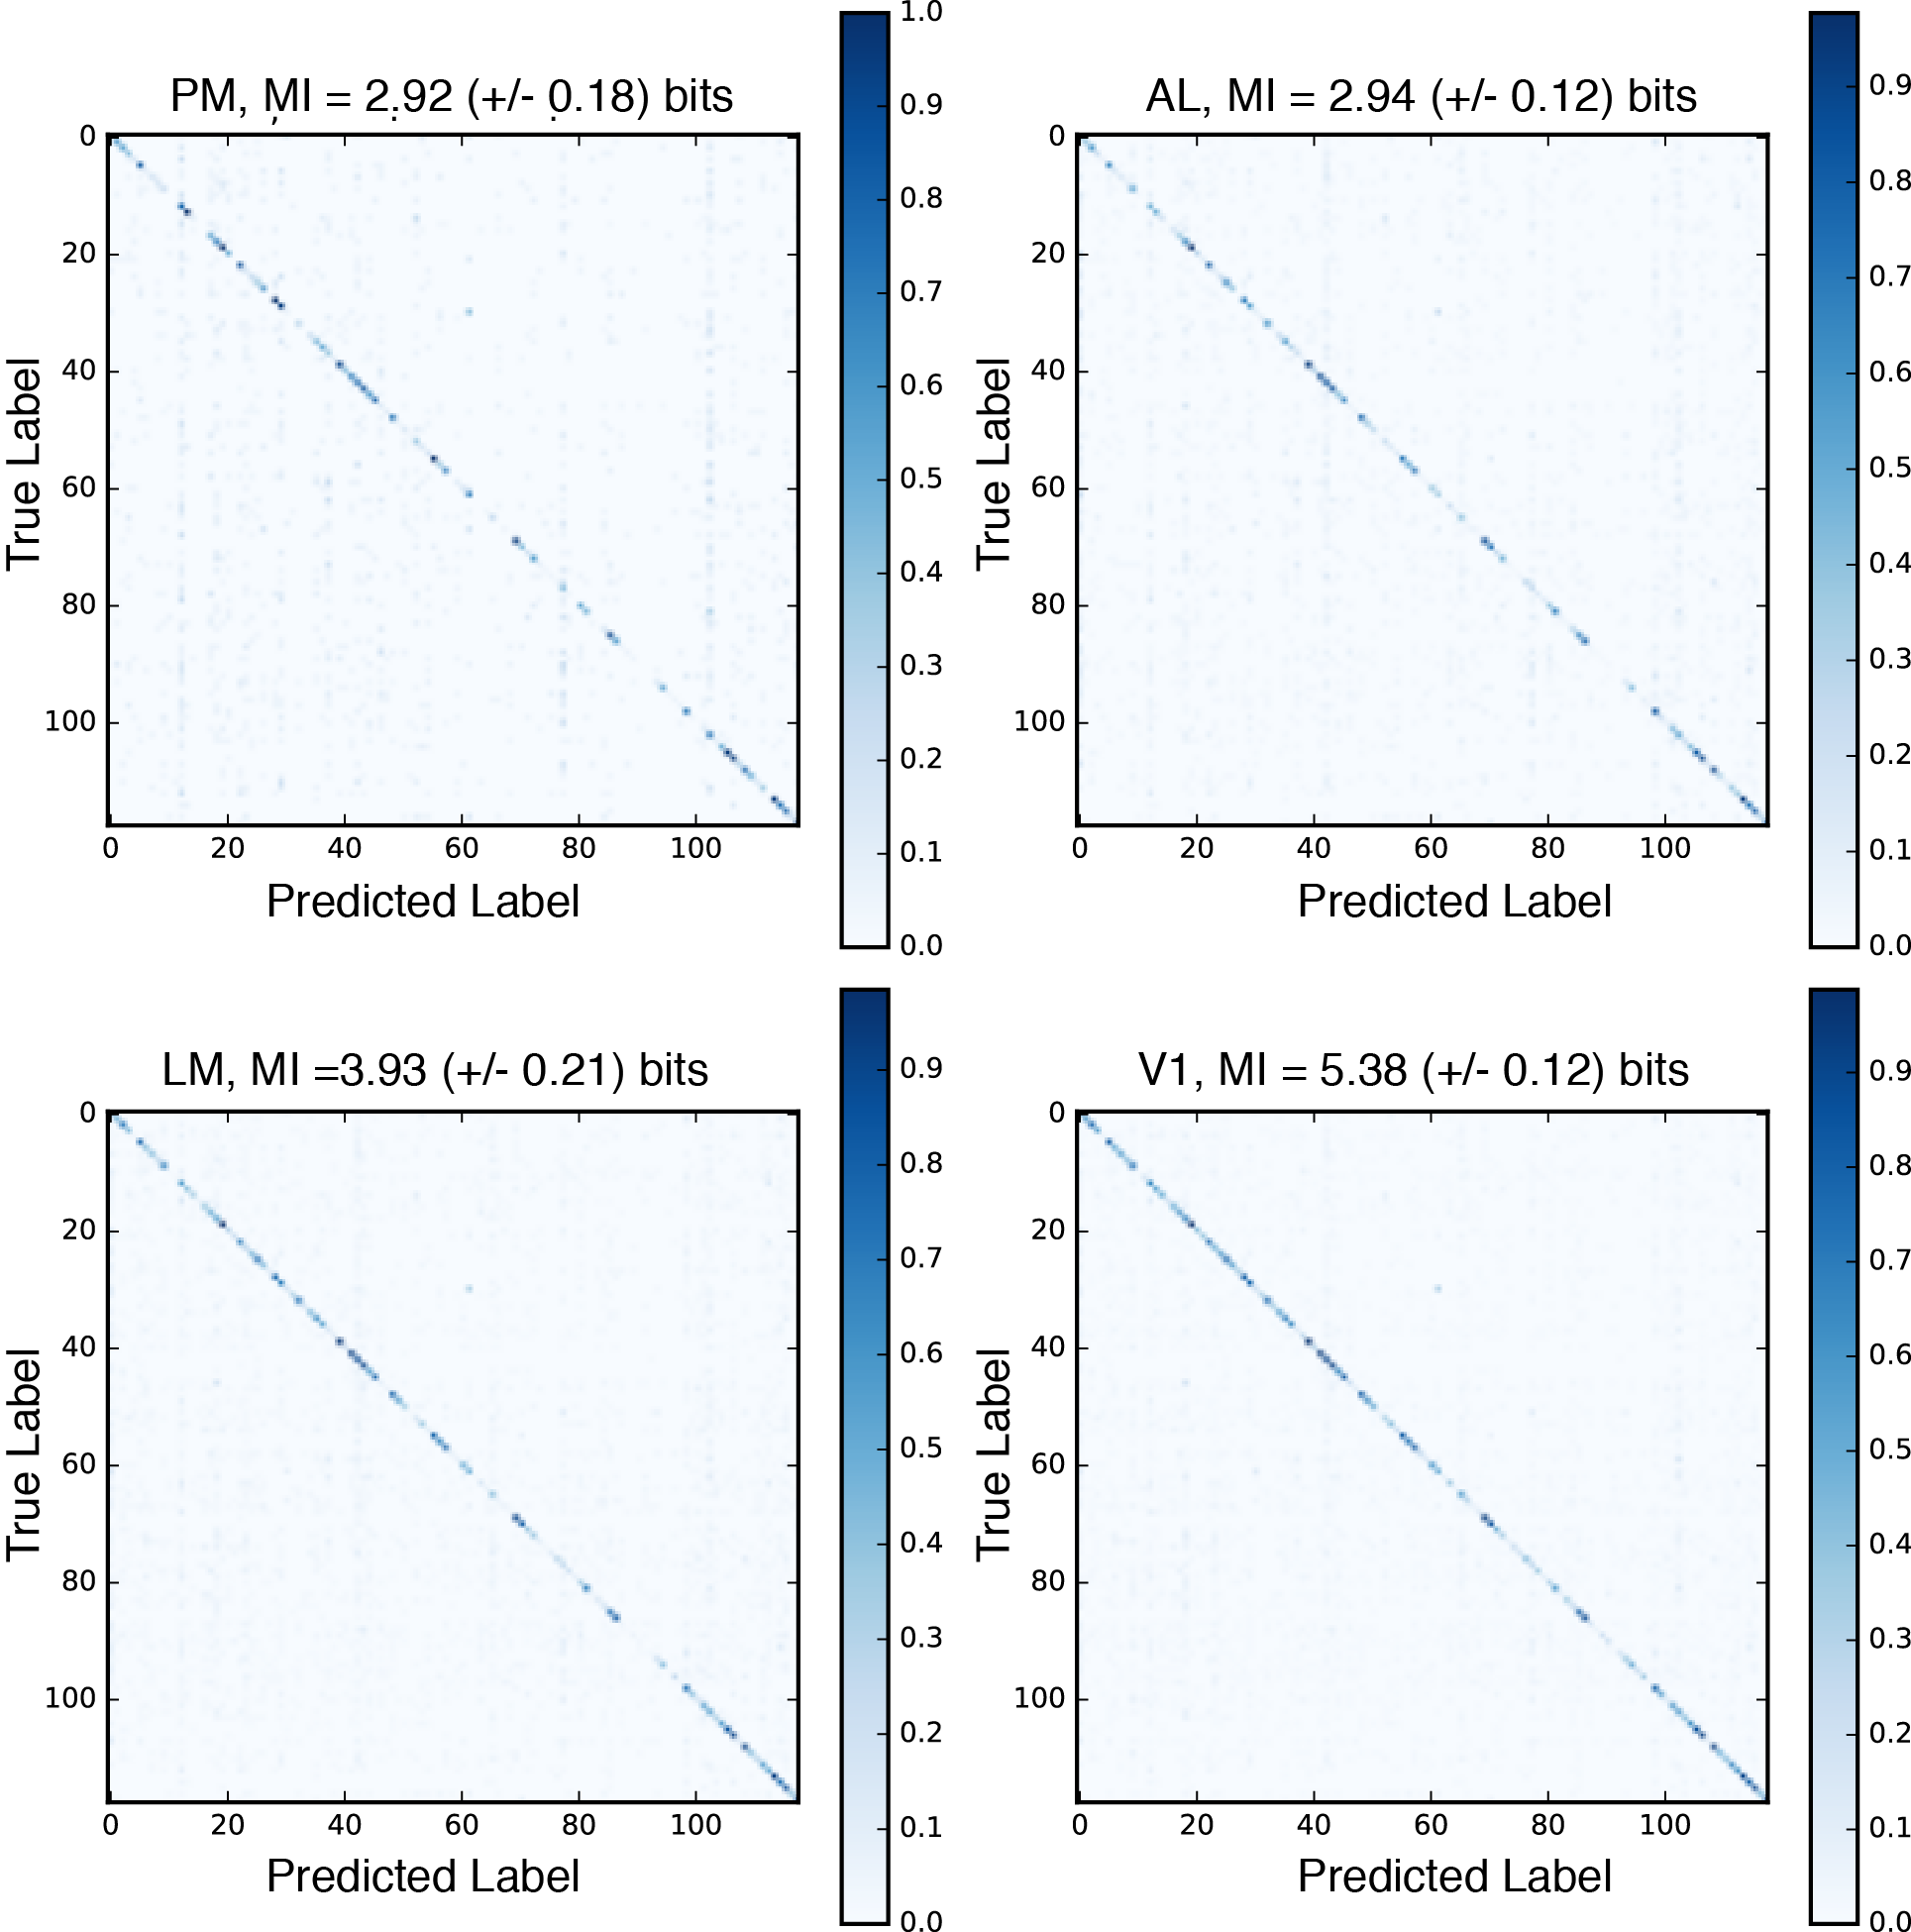
\includegraphics[width=\textwidth]{Figures/chapter5/confusion.png}
%    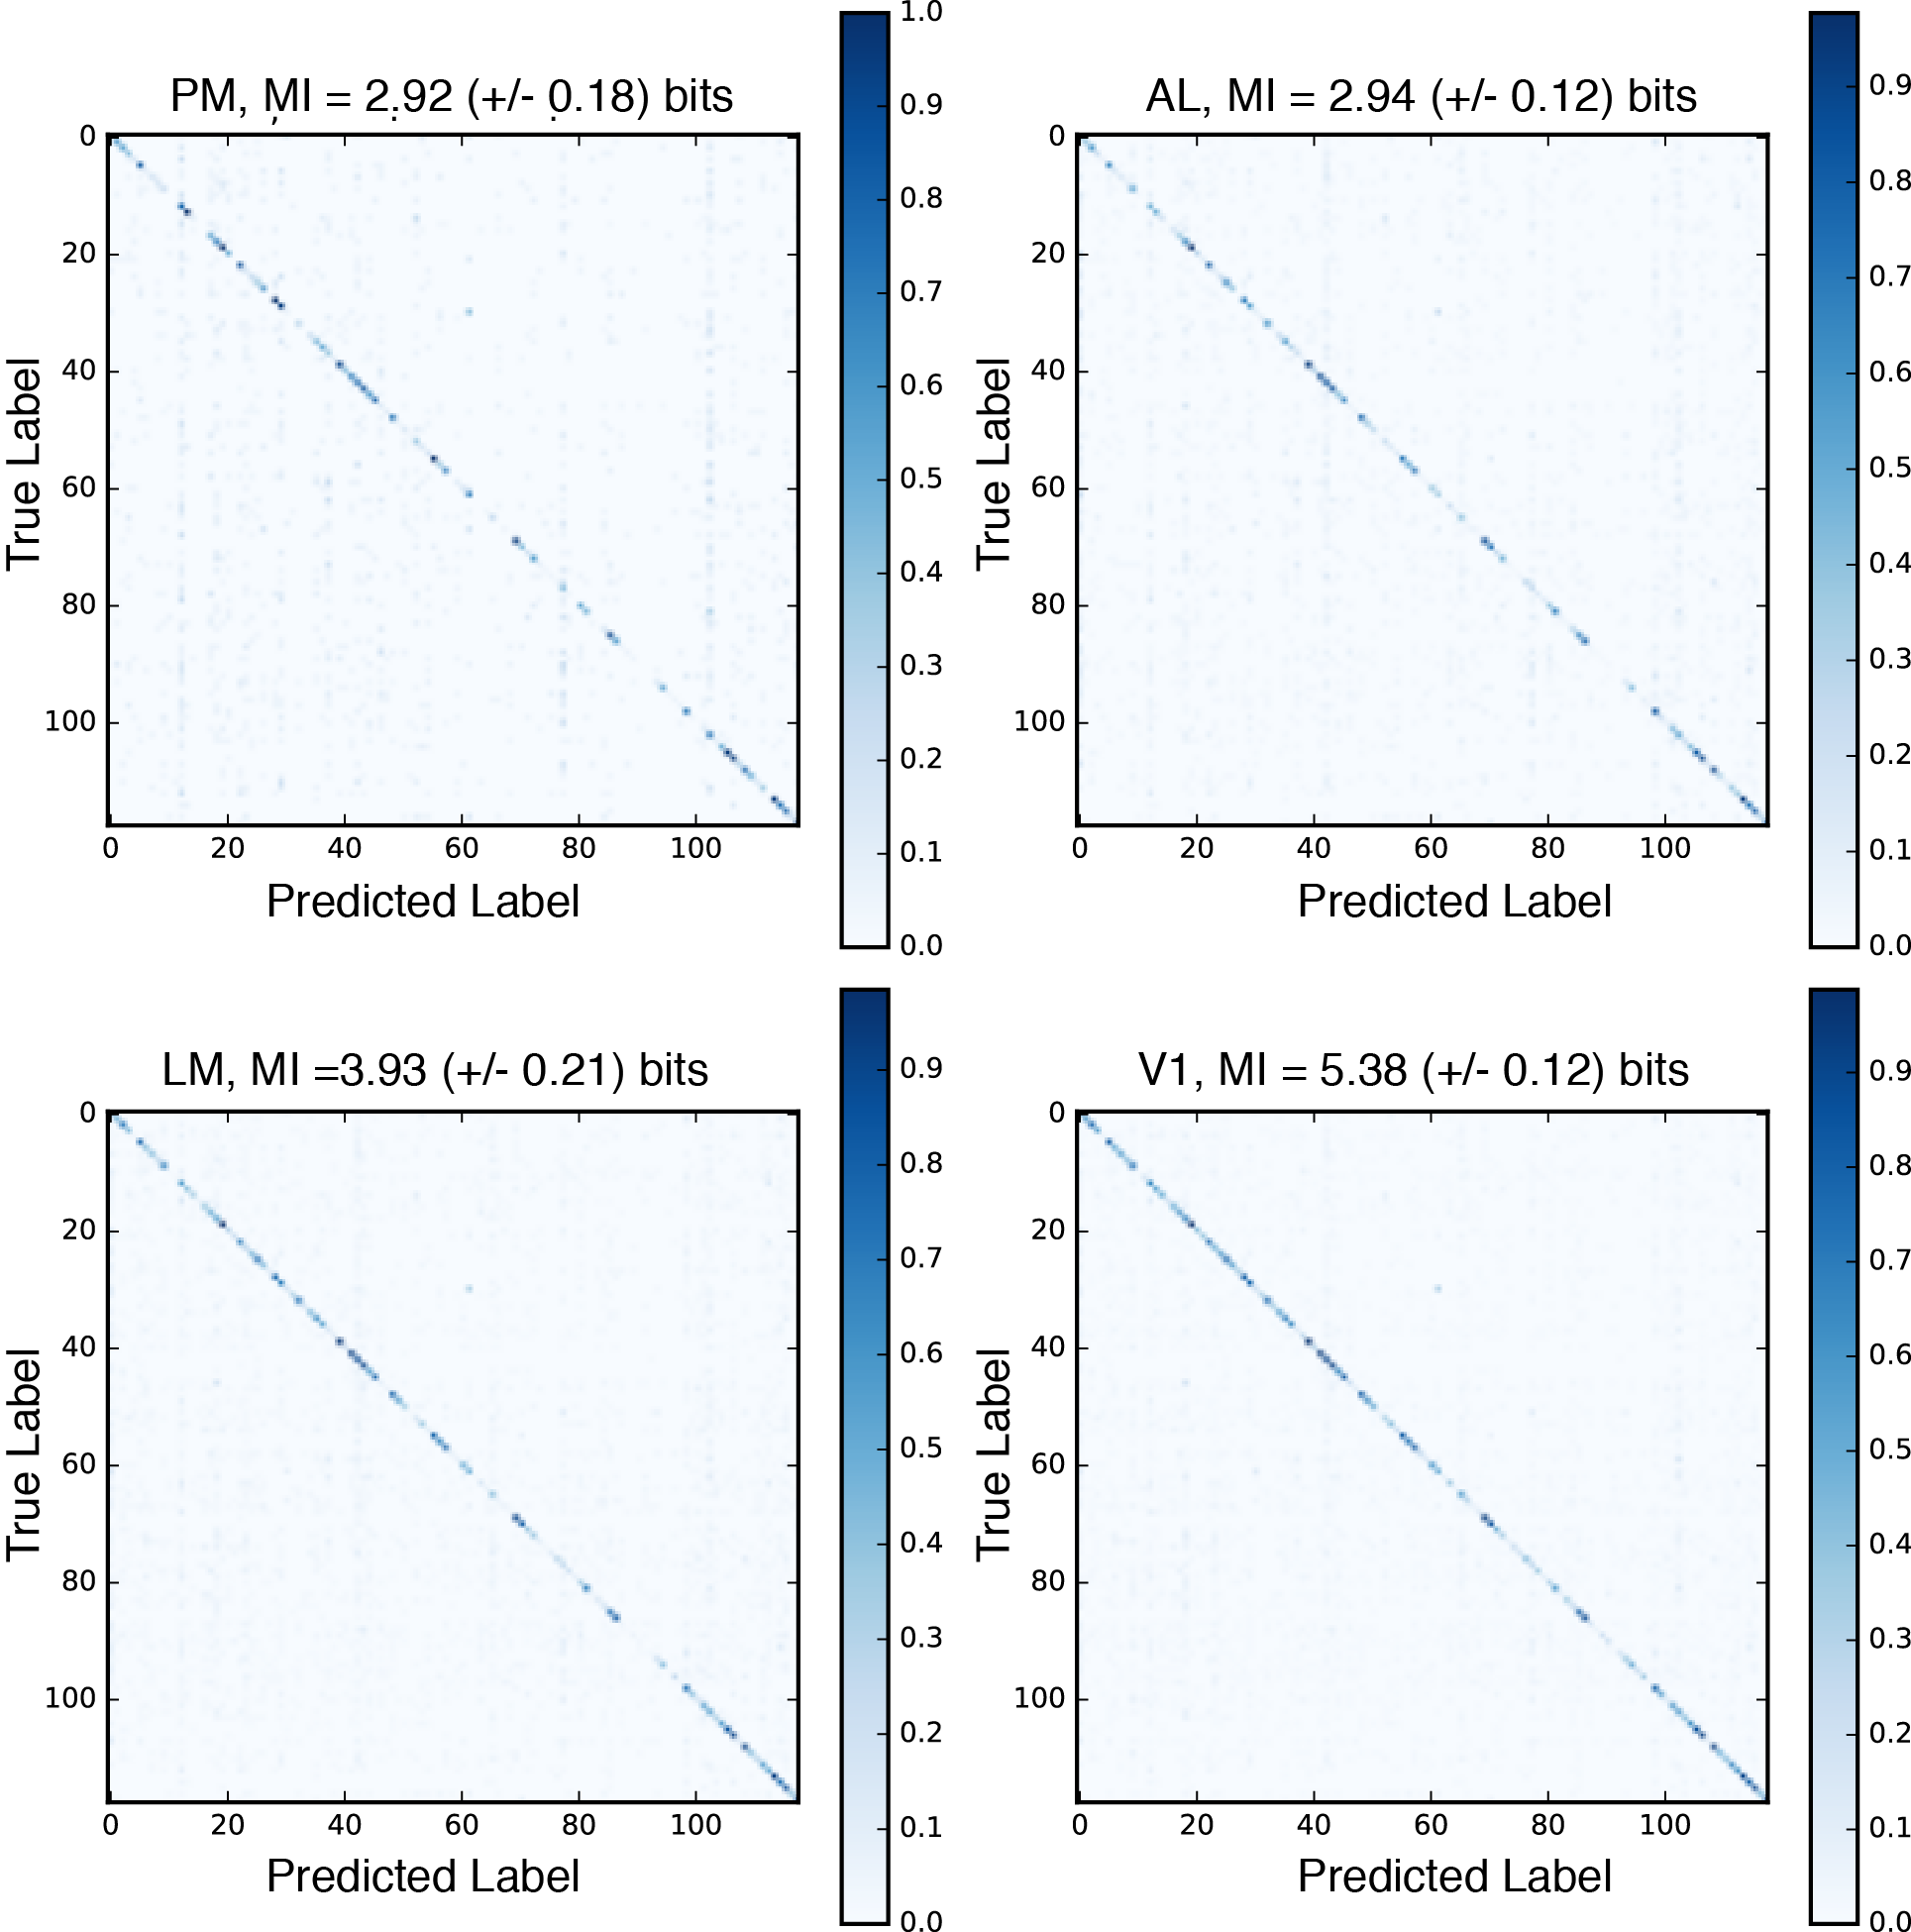
\includegraphics[scale=0.725]{Figures/chapter5/confusion.png}
  \caption[Confusion Matrix]{\textbf{Confusion Matrix} for each visual area compares decoder performance (or misclassification) for pairs of natural images. Mutual information (in bits) is reported for each confusion matrix +/- standard error of mean}
   \label{fig:confusion}
\end{figure}
%-----------------------------------------------------------------------------
\begin{figure}
  \centering
   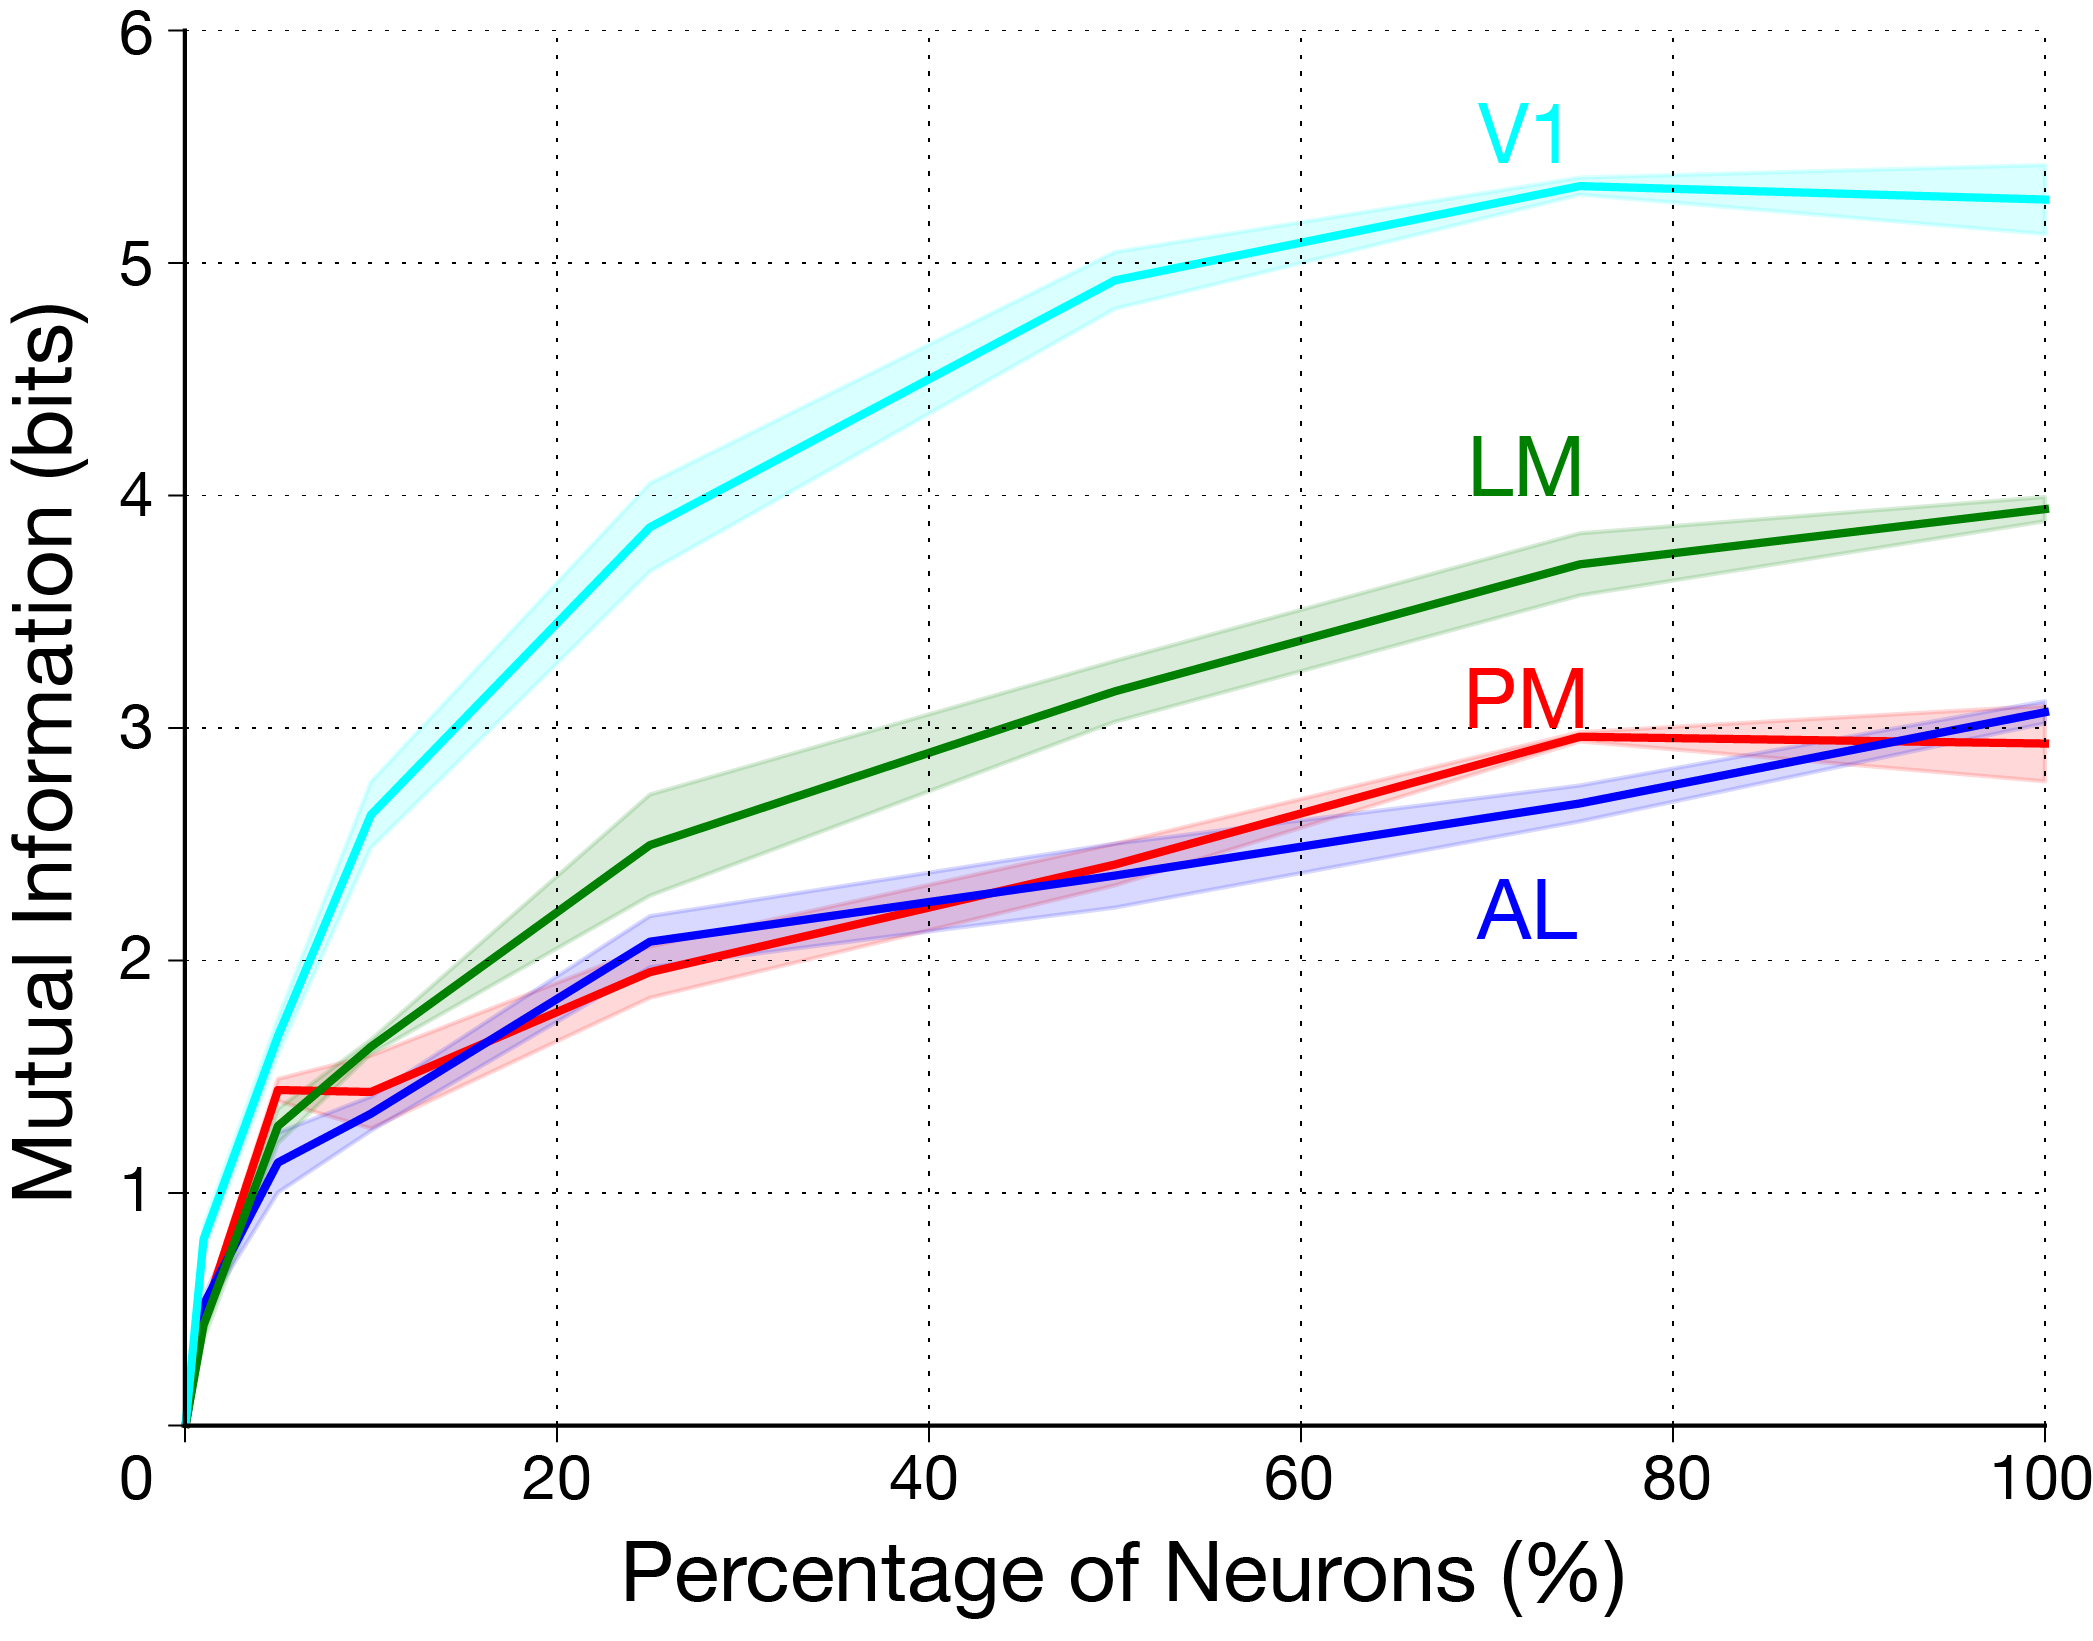
\includegraphics[width=\textwidth]{Figures/chapter5/mutual_info_pop.png}
%    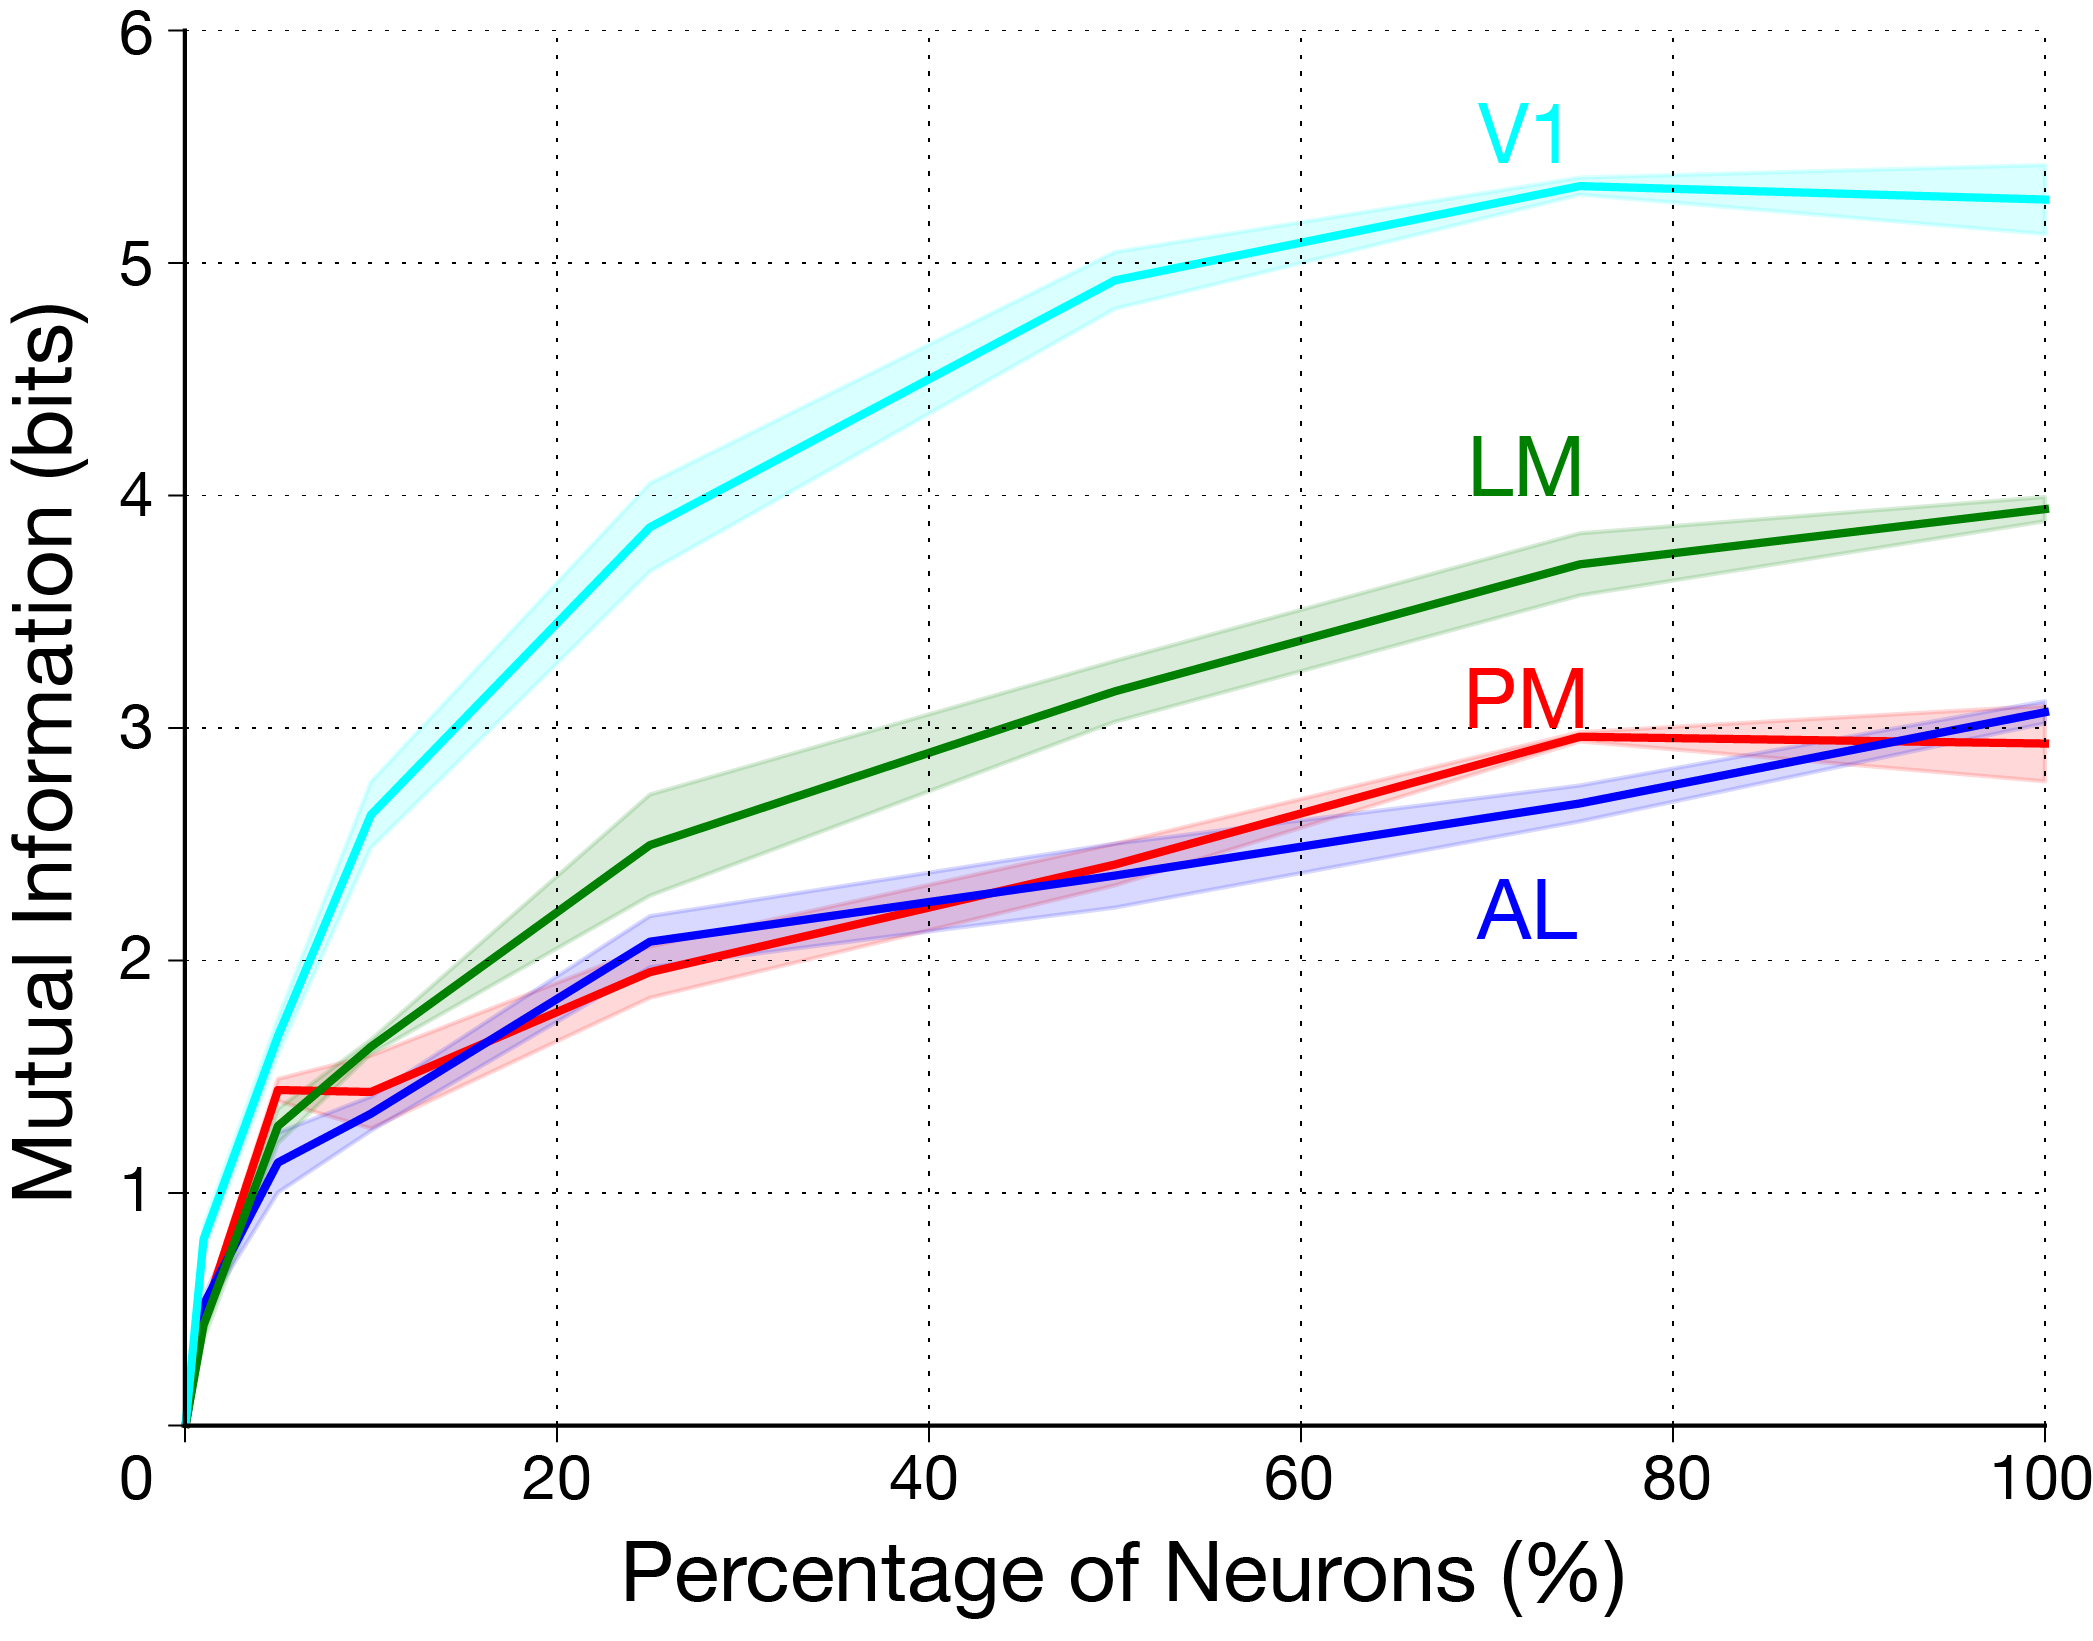
\includegraphics[scale=0.45]{Figures/chapter5/mutual_info_pop.png}
  \caption[Mutual Information Per Population Size]{\textbf{Mutual Information Per Population Size} for individual visual areas. Mutual information calculated as in Equation \ref{eq:mutualinfo}. Solid line represents mutual information. Shaded error bars represent standard error of the mean.}
   \label{fig:mutualinfopop}
\end{figure}
%-----------------------------------------------------------------------------
Next, I evaluated the information content about stimulus identity across time and whether different visual areas might achieve higher accuracy at different times from the stimulus onset. I employed two approaches to evaluate the classifier performance across time. In the first approach, I trained the decoder using the mean response from 200-300ms post-stimulus and tested the classification accuracy at different time points (Figure \ref{fig:decodetime}a). The goal was to assess whether the mean activity activity between 200-300ms also coded information about the stimulus identity at different time periods. In the second approach, I trained and tested the classifier performance at each time point independently (Figure \ref{fig:decodetime} b). Both approaches yielded identical results, with V1 exhibiting greater test accuracy over time compared to higher visual areas.\par 
%-----------------------------------------------------------------------------
\begin{figure}
  \centering
    	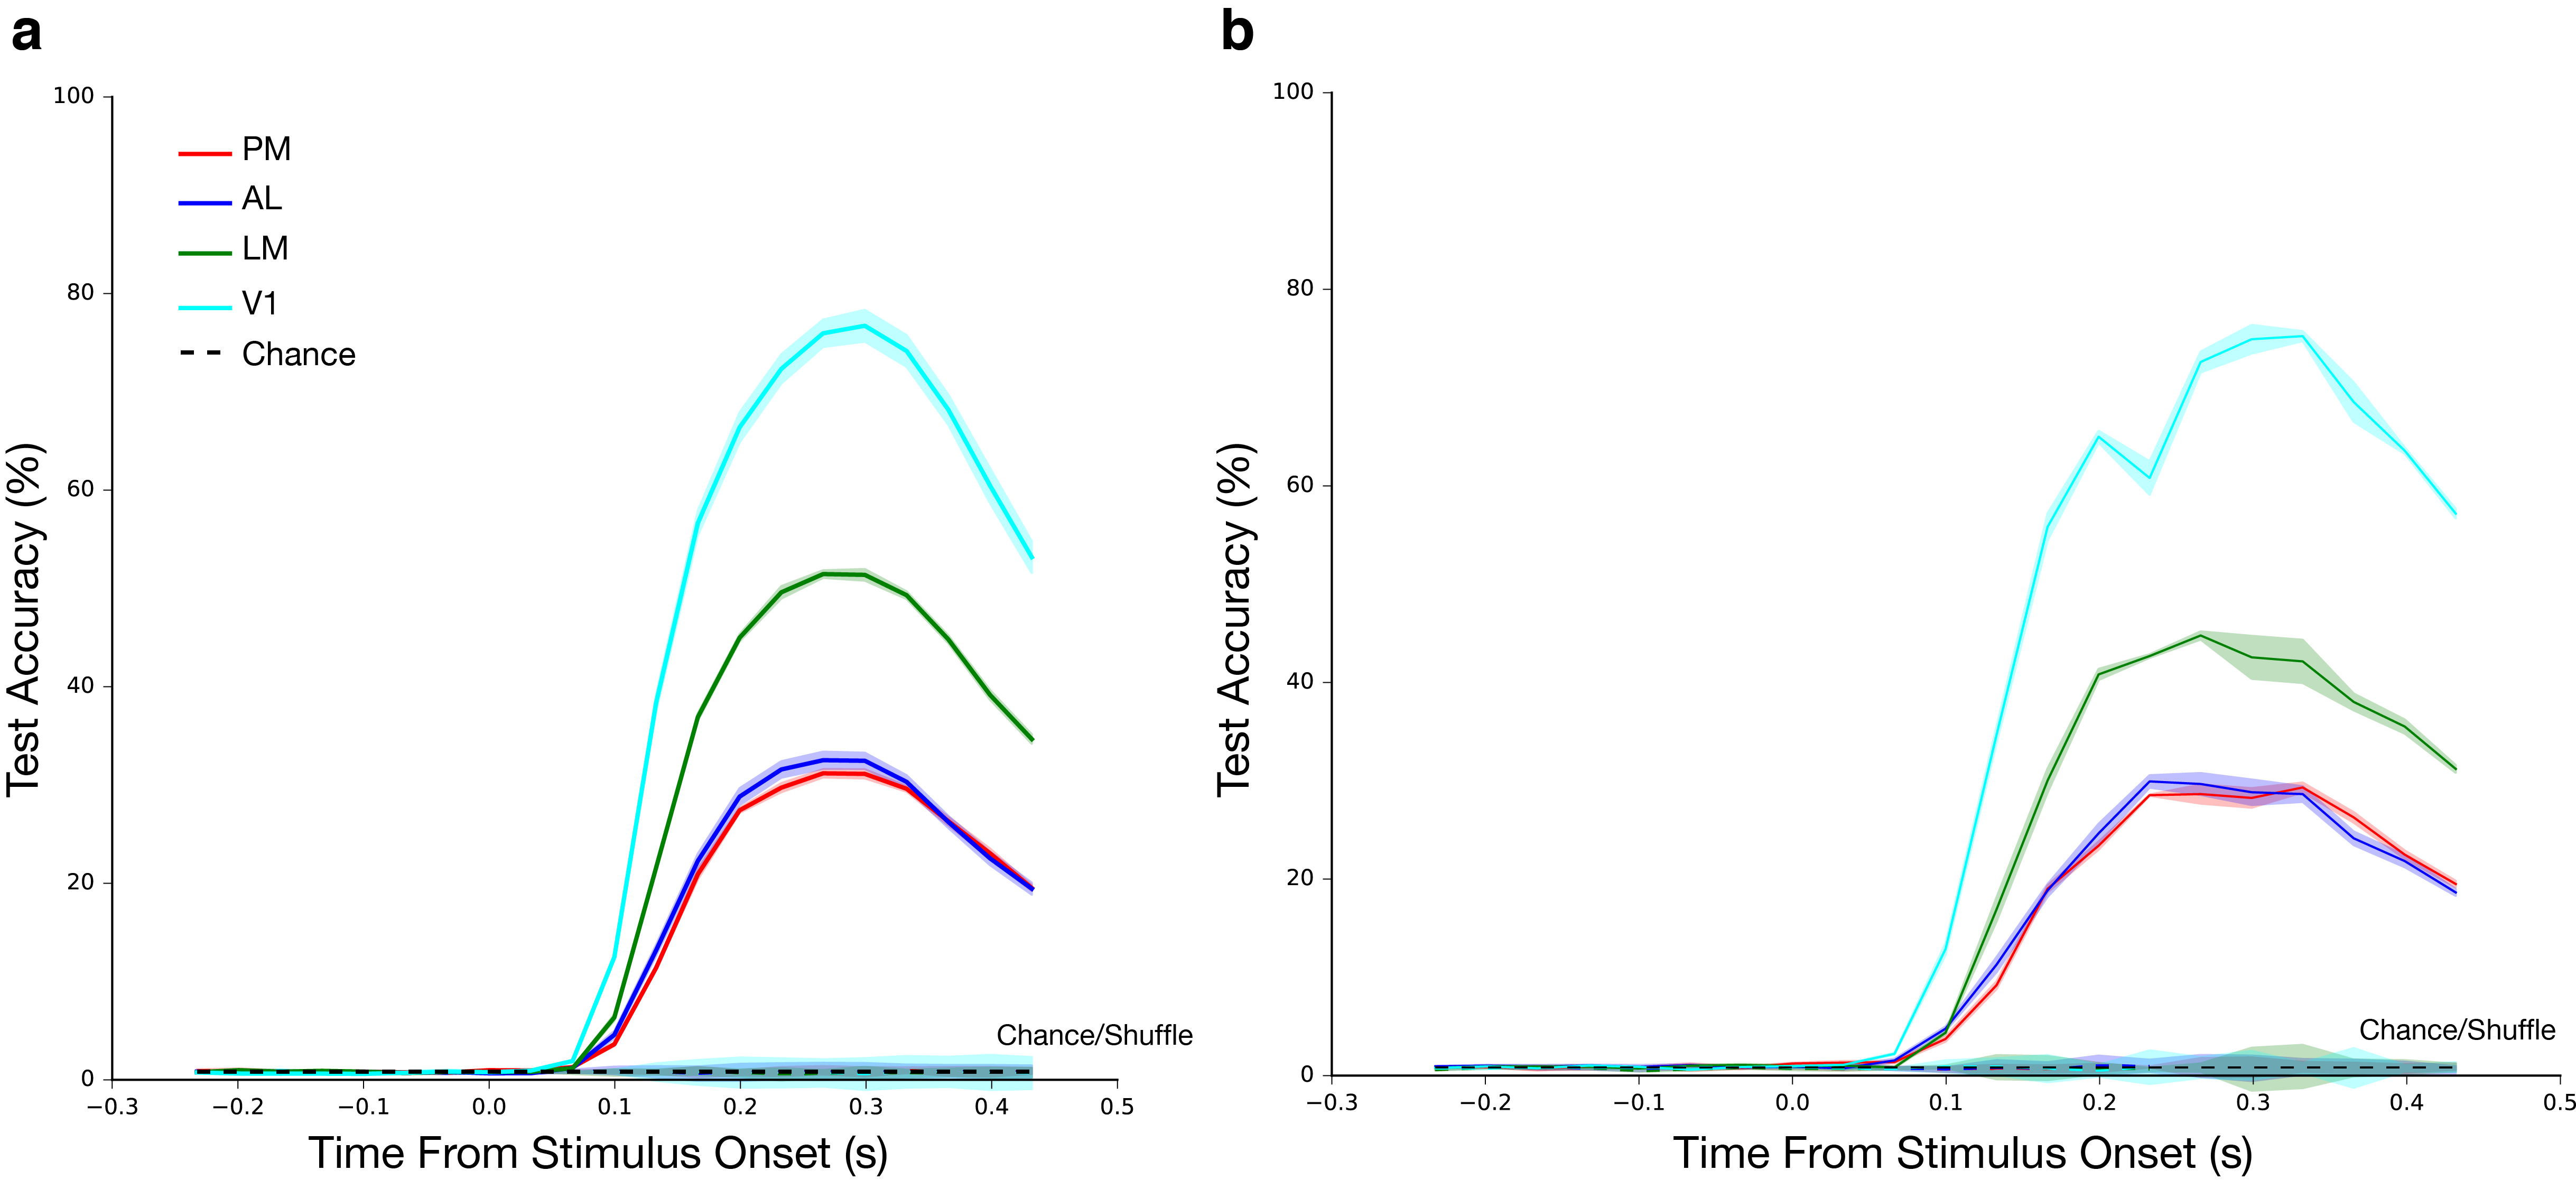
\includegraphics[width=\textwidth]{Figures/chapter5/accuracy_time.png}
%   	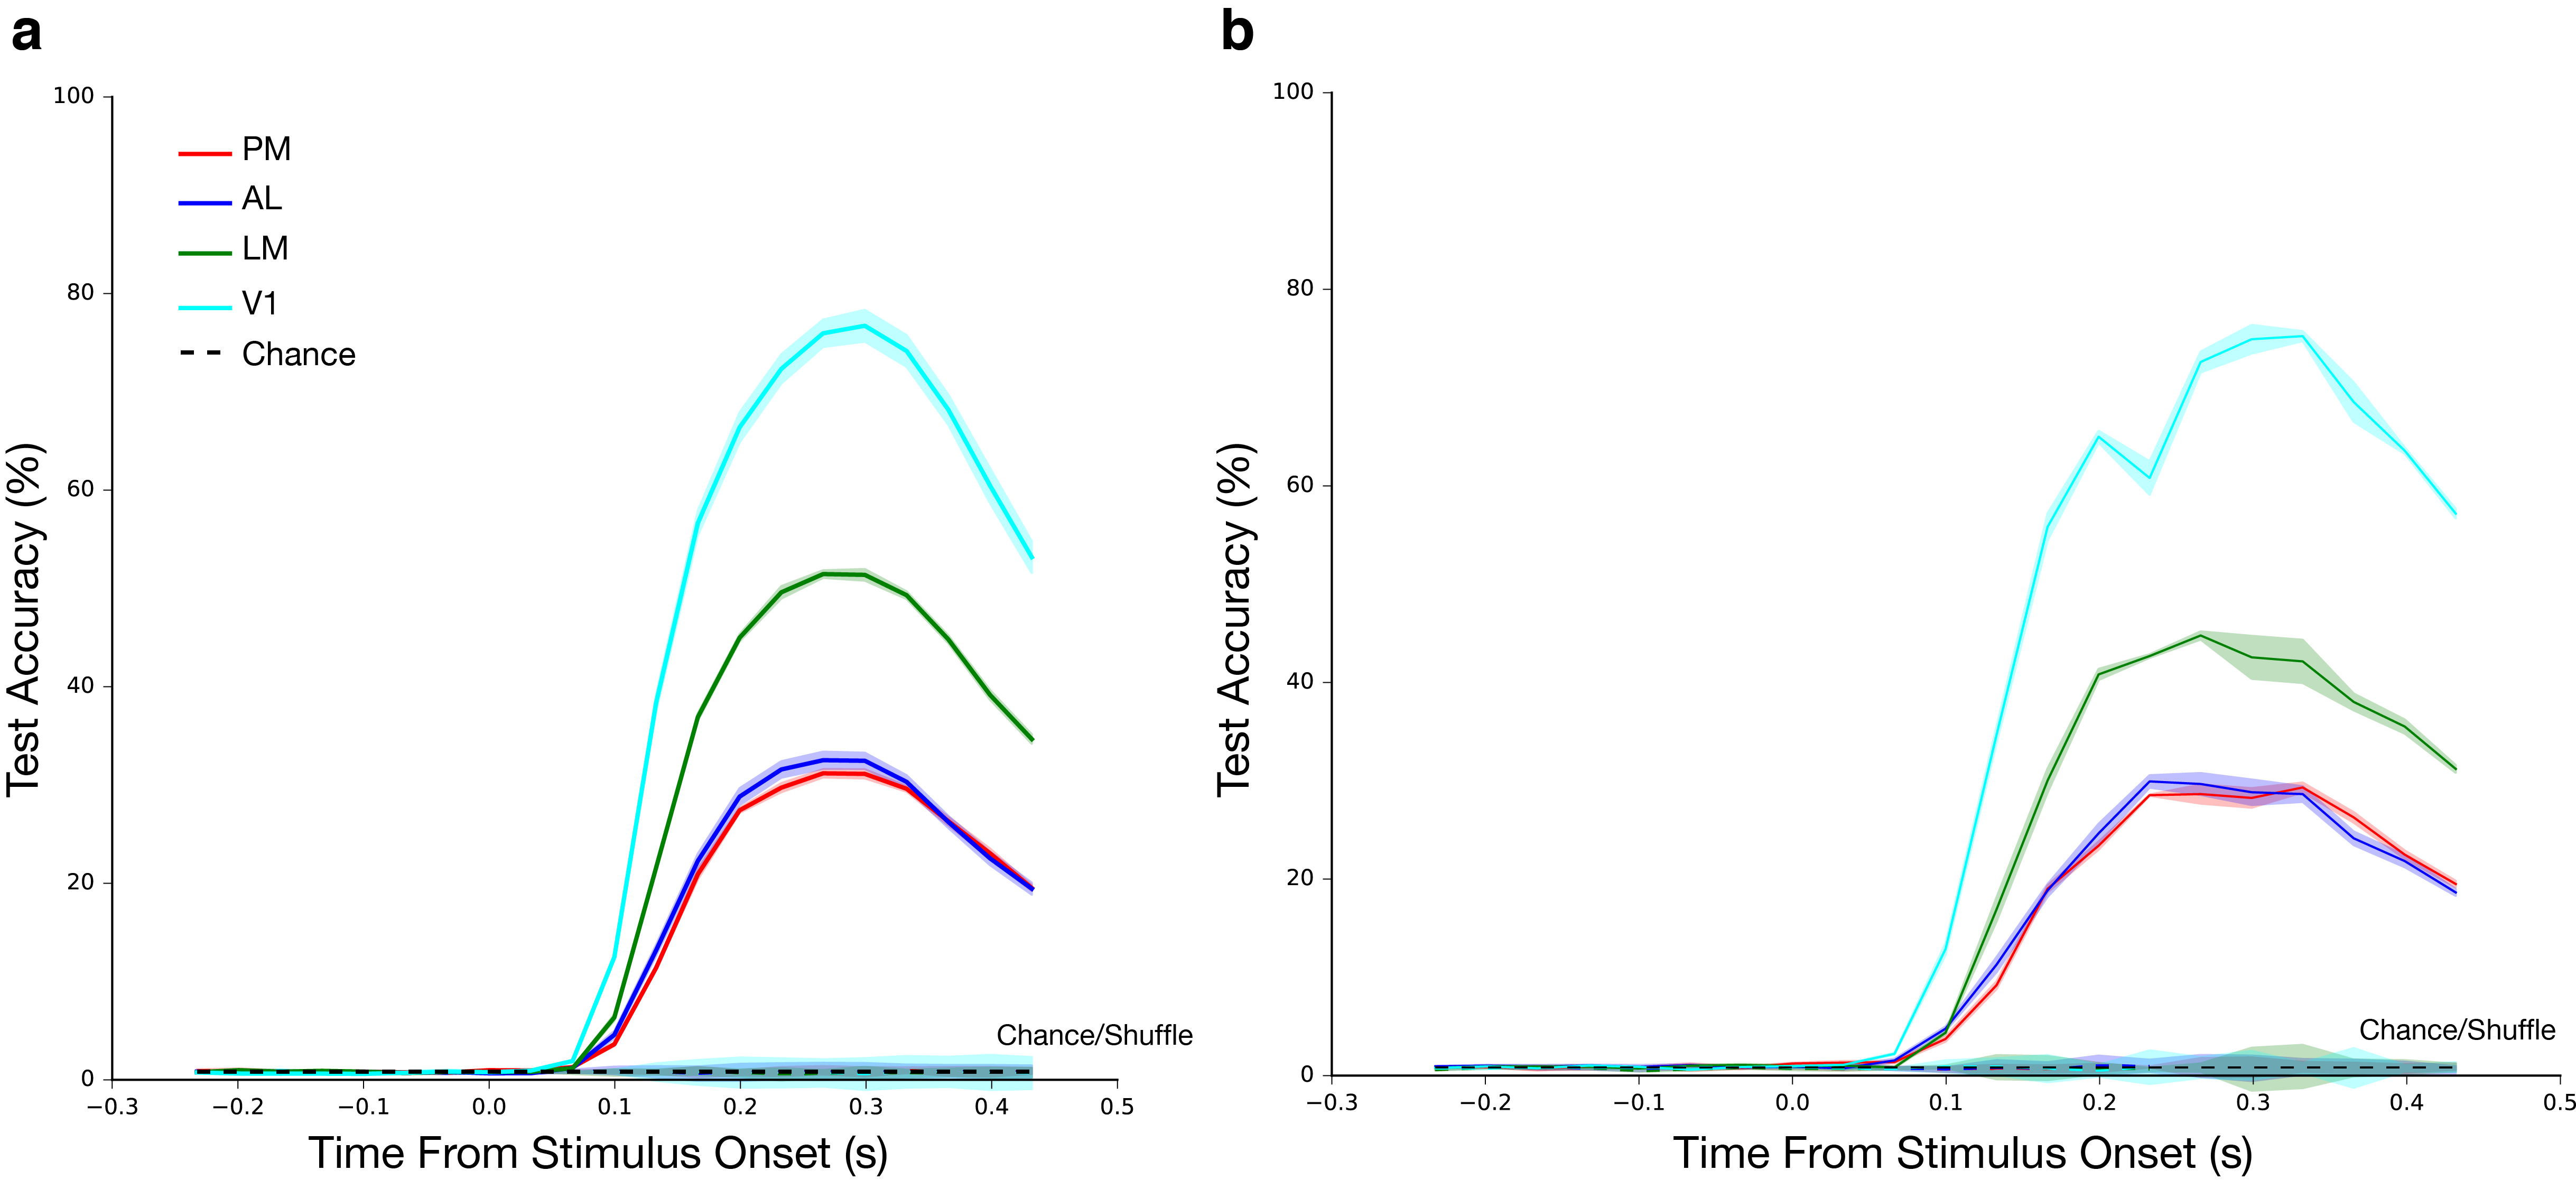
\includegraphics[scale=0.3]{Figures/chapter5/accuracy_time.png}
    \caption[Decoder Test Accuracy Over Time]{\textbf{Decoder Test Accuracy Over Time}.(a) Test accuracy of decoder trained with mean activity between 200-300ms post stimulus and tested at each time point. (b) Test accuracy for decoder trained and tested with activity at each time point. Shaded error bars represent standard error of the mean. }
  \label{fig:decodetime}
\end{figure}
%-----------------------------------------------------------------------------
The results described above included all the cells within an area, however, the data can be separated into cortical layers marked by specific cell-type markers (Table \ref{celltable}). I evaluated the performance of cortical layers within an area on decoding natural image identity (Figures \ref{fig:decodecell} and \ref{fig:decodecelltime}). For the analyses, I included 200 neurons per cell type to make an equivalent comparison across different cell types and visual areas. According to the canonical connectivity of principal cells within cortex \parencite{Harris2013}, layer 4 is the prominent recipient of thalamic input although all cortical layers receive thalamic input. Layer 2/3 receives strong projections from layer 4 and sends feedforward projections to higher cortical areas, contralateral cortices, and local projections to layer 5 while layer 5 is the main output layer with local projections to layer 2/3, ipsi- and contra-lateral cortices and the striatum. Layer 5 also receives top-down inputs from higher order brain regions and the thalamus. \par 
%-----------------------------------------------------------------------------
\begin{figure}
  \centering
   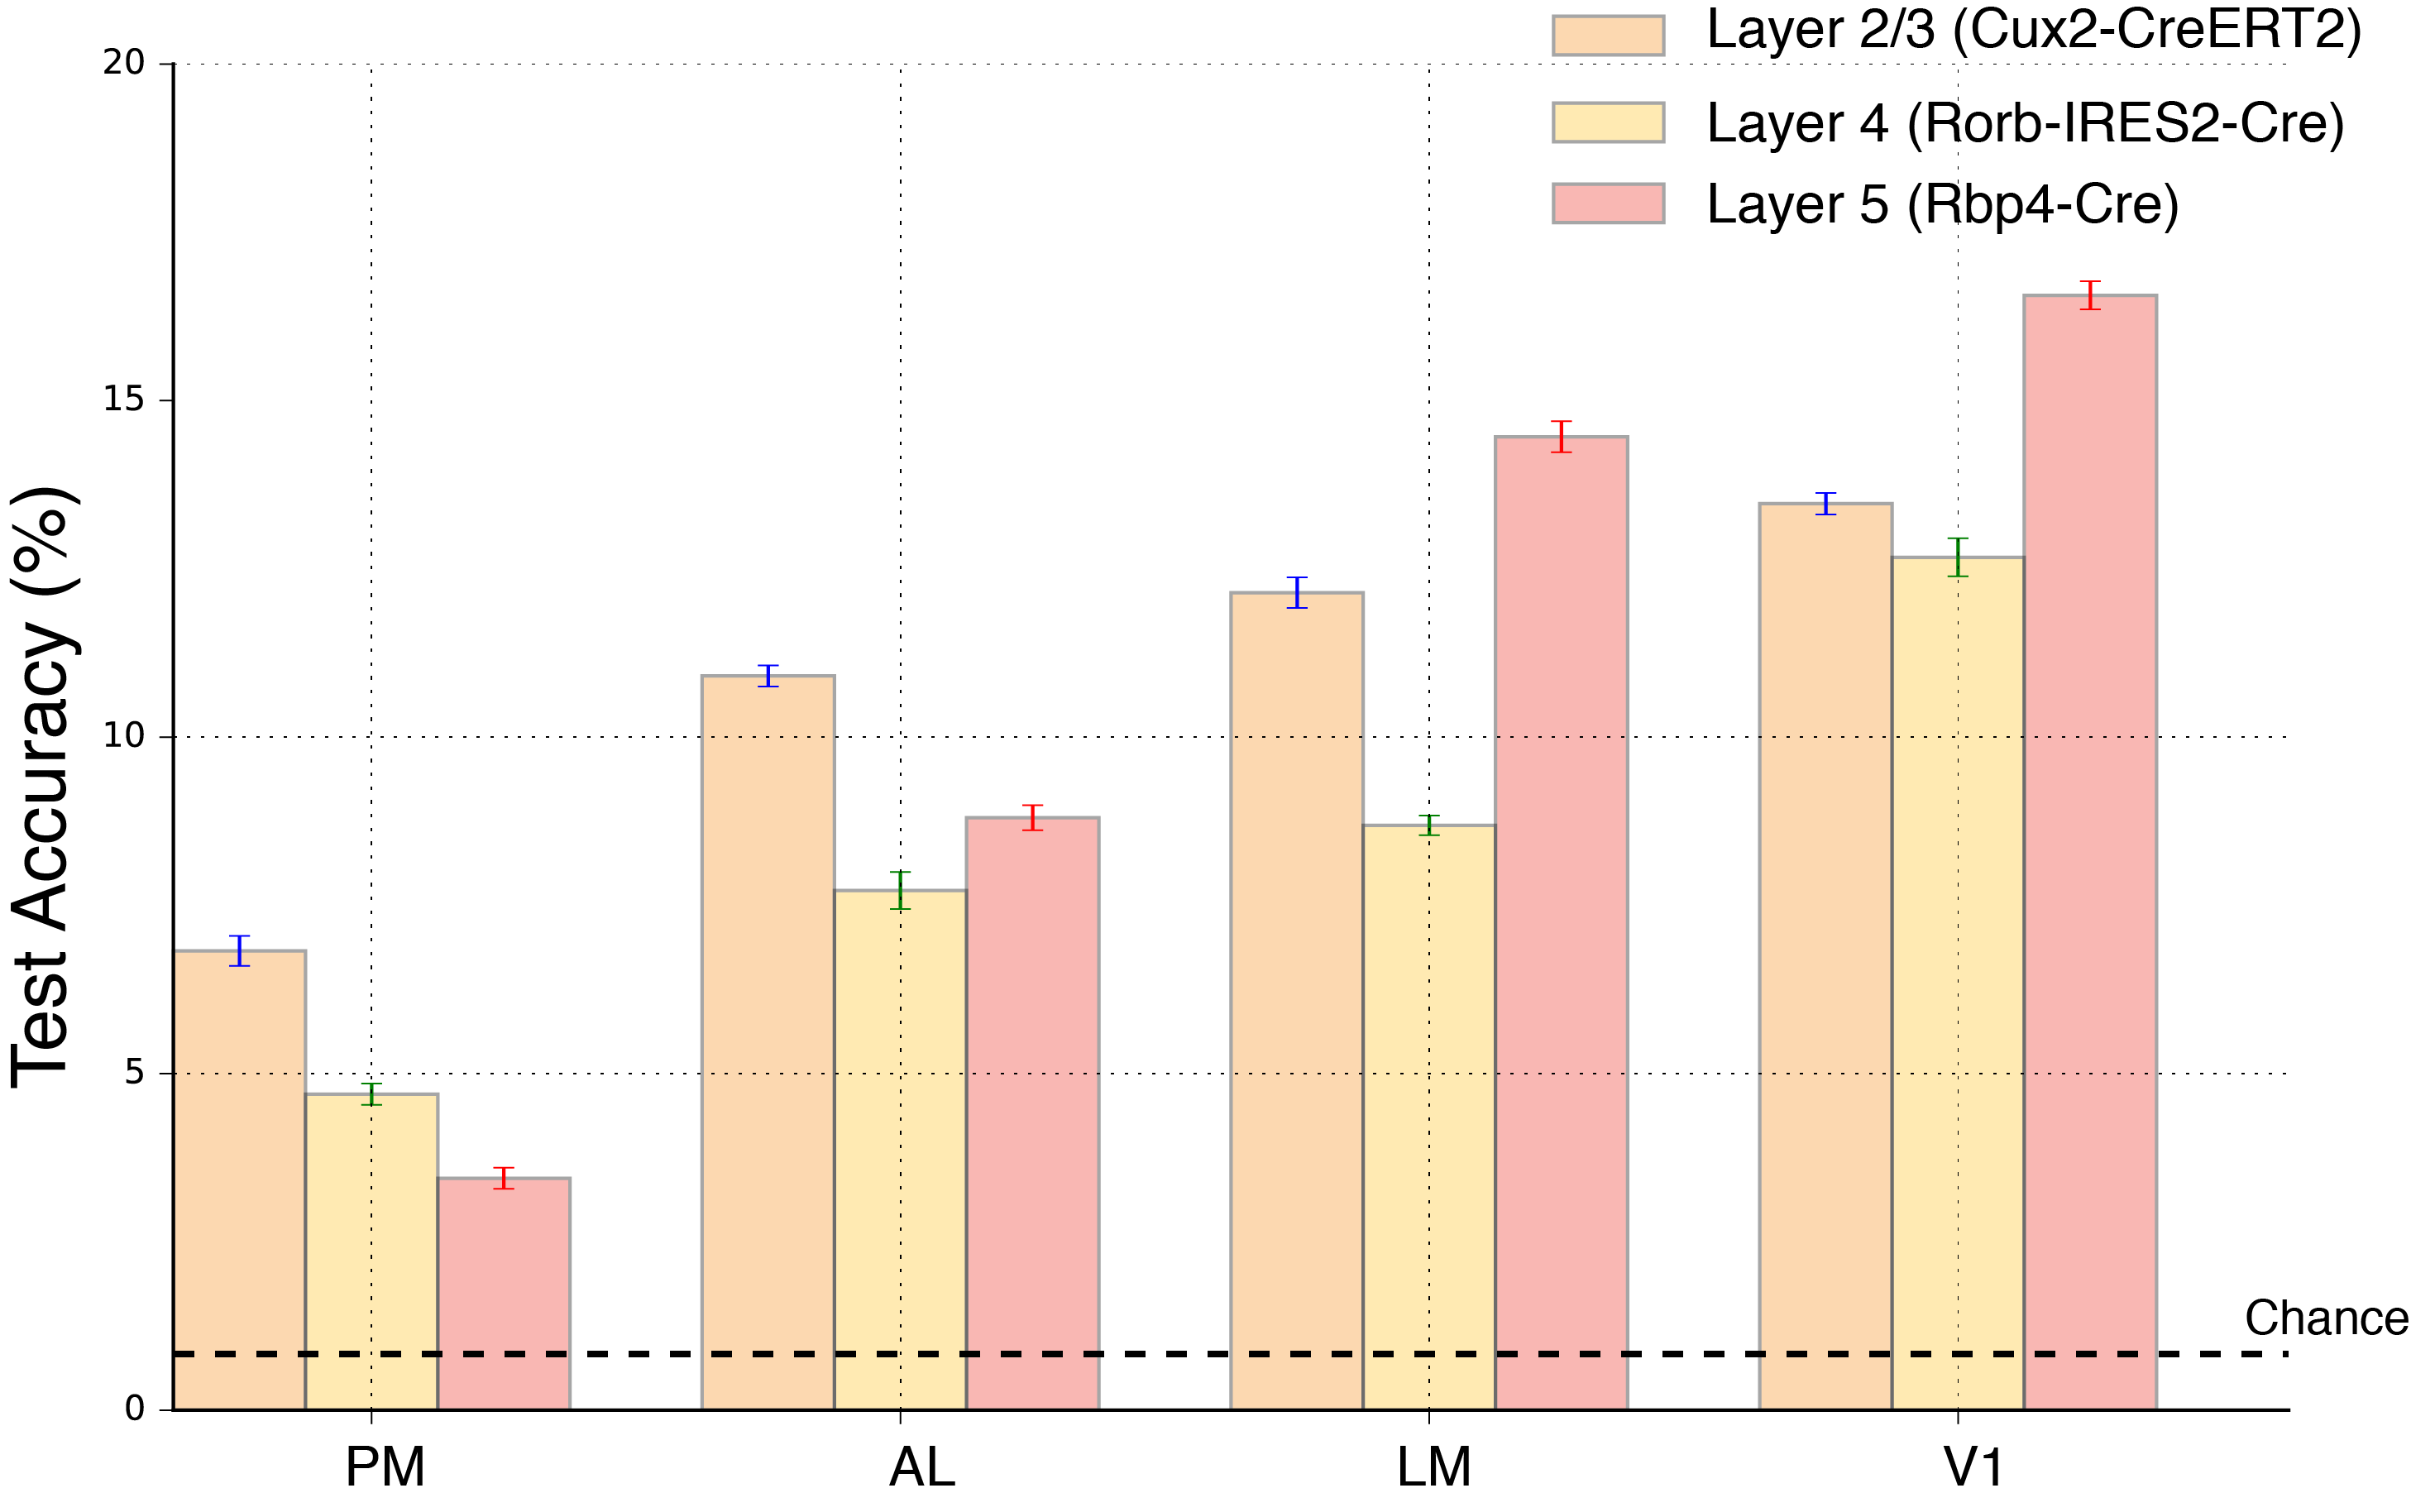
\includegraphics[width=\textwidth]{Figures/chapter5/accuracy_cell_type_200_neurons.png}
  \caption[Image Identity Accuracy Per Visual Area Per Layer-Specific Cell Type]{\textbf{Decoder Accuracy Per Visual Area Per Layer-Specific Cell Type}: Test accuracy of classifier trained on average response 200-300ms post-stimulus onset, 200 neurons per cell type. Error bars represent standard error of the mean.}
   \label{fig:decodecell}
\end{figure}
%-----------------------------------------------------------------------------
\begin{figure}
  \centering
   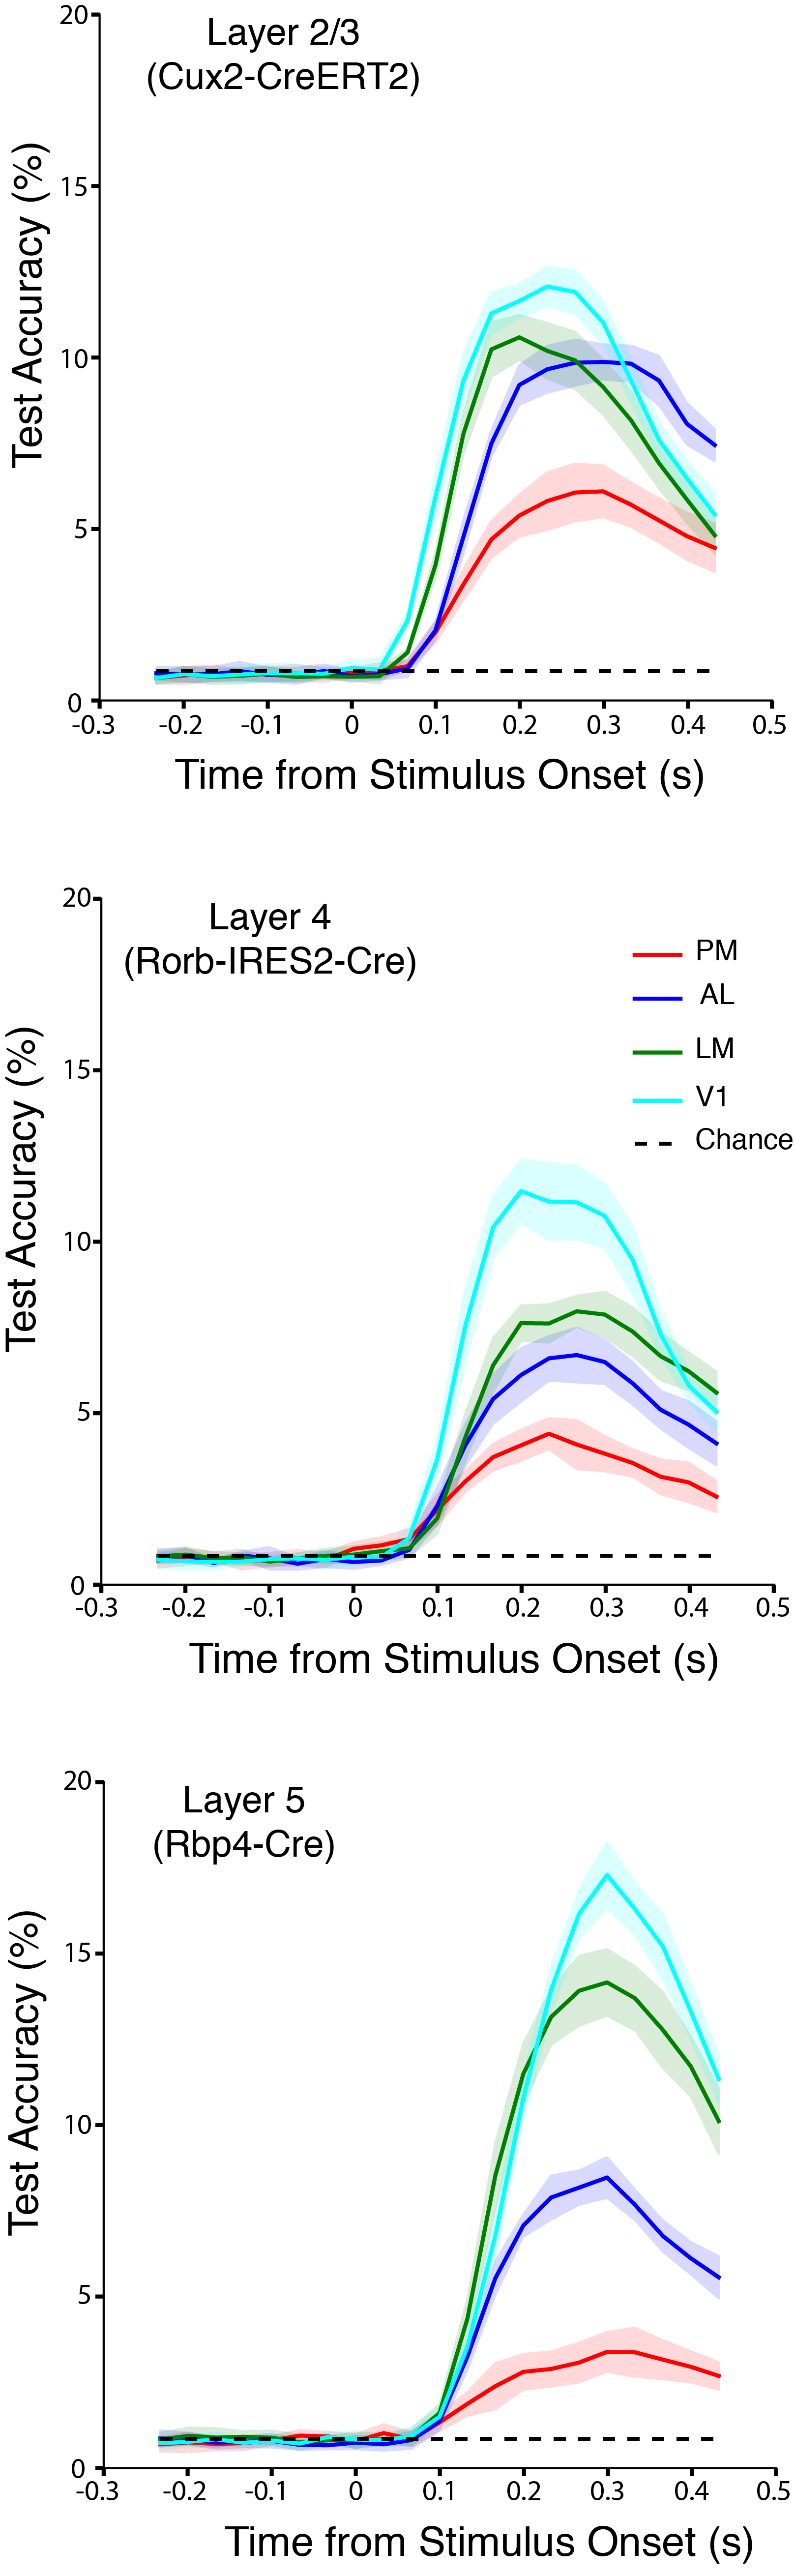
\includegraphics[width=\textwidth,height=0.8\textheight,keepaspectratio]{Figures/chapter5/accuracy_cell_type_time_200_neurons.png}
  \caption[Image Identity Accuracy Per Layer-Specific Cell Type Across Time]{\textbf{Image Identity Accuracy Per Layer-Specific Cell Type Across Time}. Test accuracy of classifier trained with mean response 200-300 ms post-stimulus onset and tested at each time point for each cell type and visual area. 200 neurons per cell type. Shaded error bars represent standard error of the mean.}
   \label{fig:decodecelltime}
\end{figure}
%-----------------------------------------------------------------------------
Although V1 achieved higher decoding performance for each cell type (Figure \ref{fig:decodecell}), there is an intriguing difference between early and higher visual areas. Layer 5 output neurons in early visual areas (V1 \& LM) achieved the highest performance in image identification, whereas in higher visual areas (AL \& PM) layer 2/3 neurons performed better than the layer 5 neurons within their respective areas. It is interesting to consider whether the reversal reflects the flow of information from early to higher visual areas. \par 

\subsection{Decoding Natural Scene Category}
%-----------------------------------------------------------------------------
\begin{figure}
  \centering
     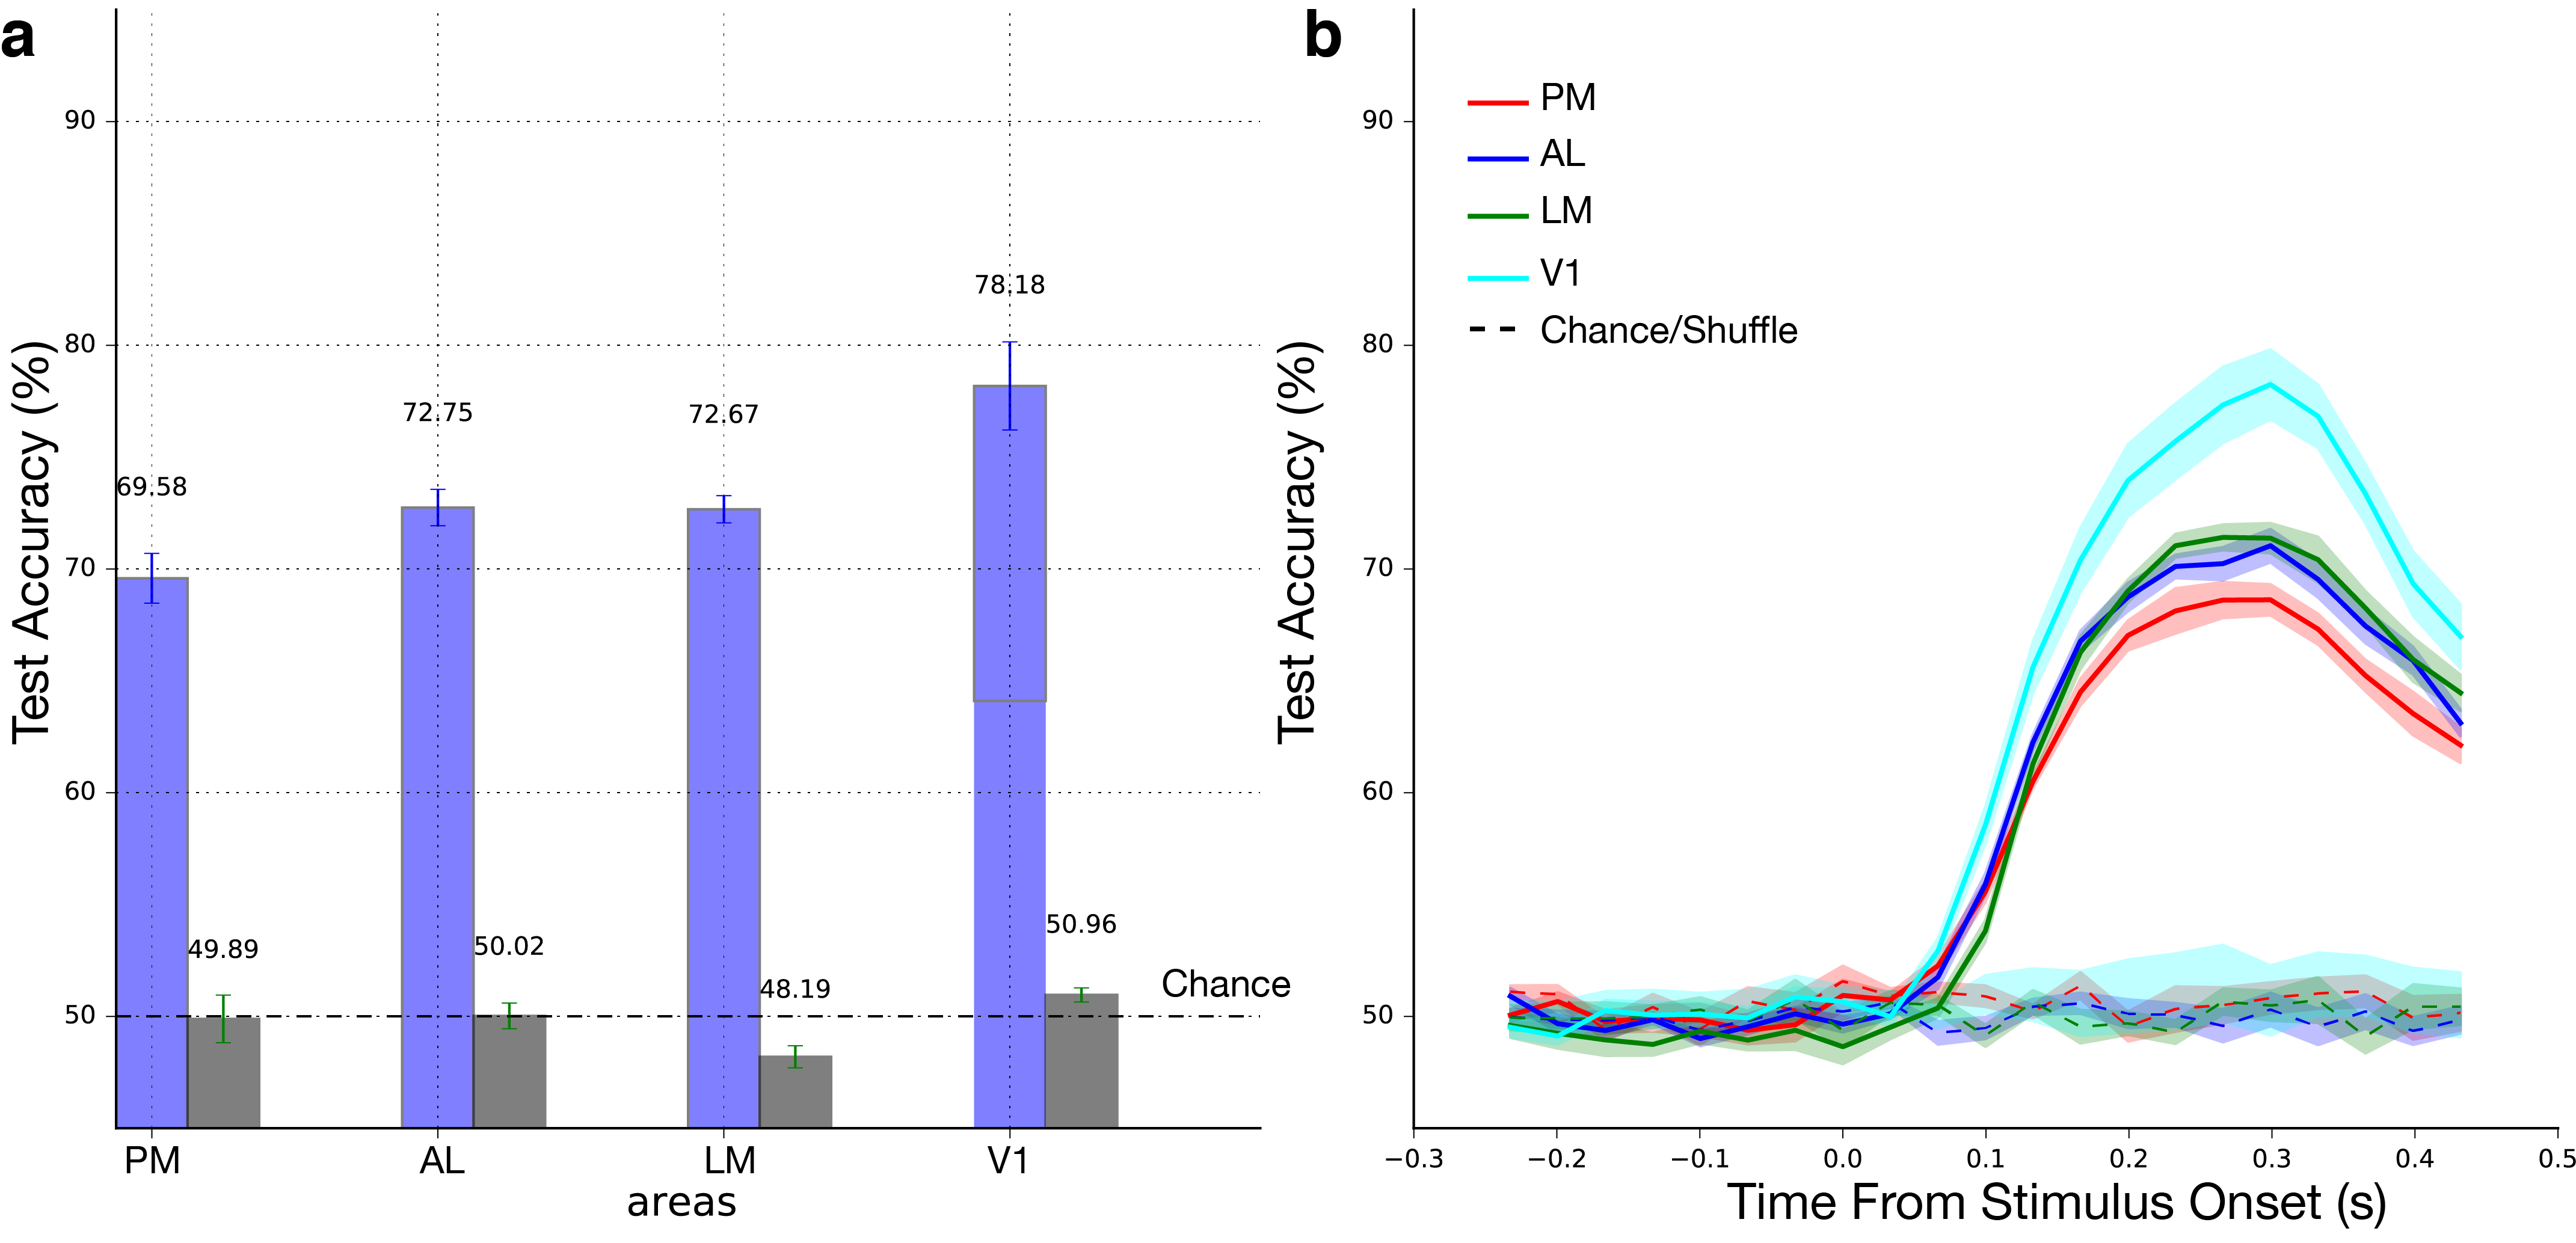
\includegraphics[width=\textwidth]{Figures/chapter5/accuracy_categorization.png}
%    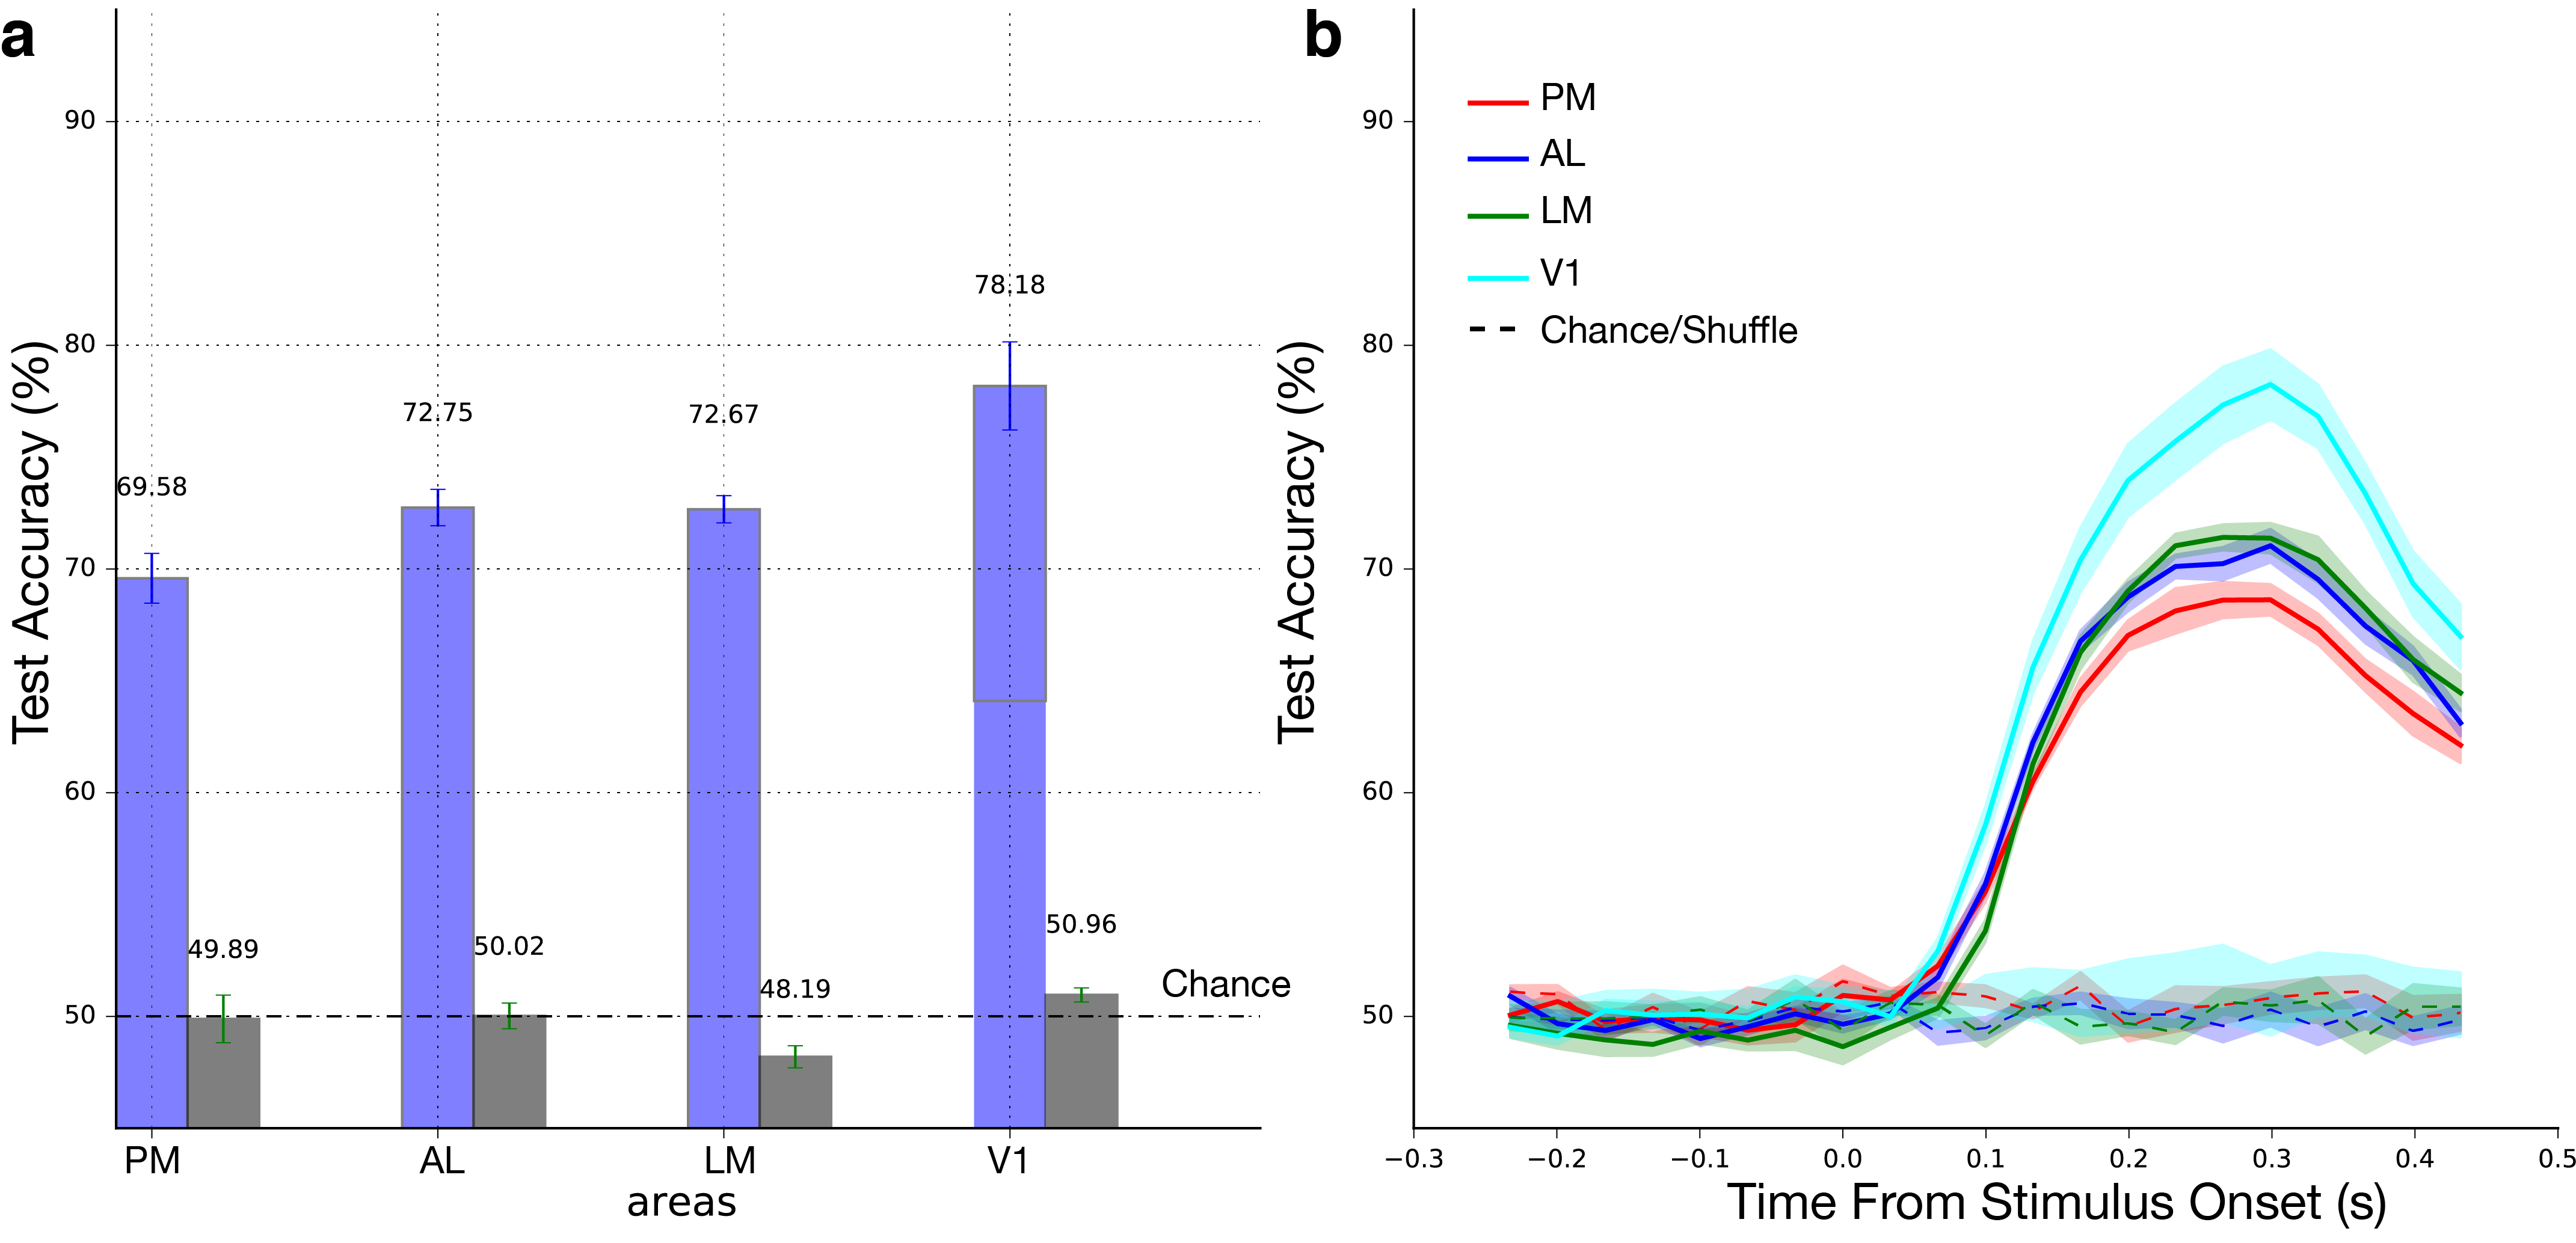
\includegraphics[scale=0.4]{Figures/chapter5/accuracy_categorization.png}
  \caption[Categorization Accuracy: Animal Vs. Non-Animal]{\textbf{Categorization Accuracy: Animal Vs. Non-Animal}. (a) Classifier test accuracy based on average response 200-300ms post-stimulus onset. Gray bars represent shuffled labeled control. Error bars represent standard error of the mean. (b) Test accuracy over time, based on classifier trained on the average response 200-300ms post stimulus onset. Dotted lines represent shuffled labeled control. Shaded error bars represent standard error of the mean.}
   \label{fig:decodecategory}
\end{figure}
%-----------------------------------------------------------------------------
Given the neural responses from visual areas perform well above chance on a natural image identity task, the next question I asked was whether the neural responses could categorize the natural images and whether higher visual area (AL \& PM) would achieve higher performance over early visual areas. The natural images were divided into two groups based on whether an animal was present in the image. A linear classifier was trained for each area to categorize the images into one of two classes. Categorization performance across visual areas was above chance (50\%) and very similar to each, with V1 achieving slightly higher accuracy (Figure \ref{fig:decodecategory}).  

\section{Discussion}
Although the observation that mouse V1 can discriminate natural images is consistent with observations from a previous study from \textcite{Kampa2011}, it is remarkable that V1 \emph{linearly} distinguishes natural images at a greater accuracy than higher visual areas. This observation is in contrast with the seminal view of hierarchical visual processing, which suggests progressive reconstruction of the image from basic low-level representations from the earliest stage to the highest stage in cortex where objects and scene layouts are represented. Embedded in this viewpoint is increased linear separability of the neural representations of the visual image (or object) along the hierarchy \parencite{Rust2010a,Pagan2013}. The primary evidence for hierarchical processing in rodent brains originates from anatomical connectivity \parencite{Coogan1993,Wang2012,DSouza2016}, however it has not yet been established whether a functional visual processing hierarchy exists in the mouse brain in a form similar to the hierarchical and specialized visual processing modules found in the primate brain \parencite{Felleman1991}. \par 

\textcite{Oliva2001} proposed an alternate computational model for scene perception, which states that scenes can be recognized based on holistic (or low-dimensional) descriptions of the scene, also known as the spatial envelope. In this model, scenes can be recognized by linear combinations of low-level features of the image. Further, \textcite{Torralba2003} observed that the spatial properties of the scene and scene category are correlated with second-order statistics of the image and the spatial arrangement of structures in the scene. The model could explain the high decoding accuracy of mouse V1 observed in this chapter. V1 is a low-level feature detector that responds to edges, orientation, and contrast \parencite{Niell2008a,Glickfeld2013b}. Consistent with the computational model proposed by \textcite{Oliva2001}, \textcite{Rikhye2015} recently reported that neurons in mouse V1 use second-order image statistics (ie. spatial correlations) to process natural scenes. \par 

Receptive field (RF) sizes in the mouse visual cortex mirror those found in primates, where RF size increases from early to late visual areas to a size that covers a visual hemifield \parencite{Wang2007}. Since V1 neurons have smaller RFs, V1 could sample the image more densely and resolve more of than image than higher visual areas. Related to the smaller RF sizes in V1, the secondary visual areas have incomplete coverage of visual space \parencite{Garrett2014,Zhuang2017}. Given that individual mouse secondary visual areas could only sample a portion of the visual scene, multiple secondary visual areas might combine resources to gain full access to the visual scene and potentially outperform V1. One way to test this would be to combine neurons from pairs of areas with non-overlapping visual coverage, for example LM \& PM or AL. Then, one could run the classifier analysis combining neurons from areas LM and PM or AL and compare this combined multi-area performance to that of V1.\par 

A major caveat of this study is that the observations are potentially correlated with the quality of the imaging data. The data was collected from each area individually, across different mice. It is not clear whether the quality of the responses is homogeneous across visual areas and depths. For example, higher visual areas PM \& AL may have different imaging quality than V1, which is larger and has more active neurons. The results from this study will greatly benefit from electrical recordings under the same conditions. In the interim, one could degrade the signal quality from V1 by adding noise to the dF/F signal and compare the decode performance. A conceptually similar approach would be to infer spikes via deconvolution methods \parencite{Vogelstein2010}, compare spikes across areas and remove spikes to vary the signal-to-noise ratio. It would also be useful to simultaneously record from multiple visual areas within the same animal.\par 

In the analyses presented in this chapter, I evaluated the decoding accuracy of identifying natural image in awake, passive animals. Future experiments would benefit from testing whether the V1 dominance in natural scene identification persists even when mice are actively engaged in a behavioral task that requires natural scene categorization. Although V1 achieved highest performance in linearly distinguishing between natural images, the neural activity pattern could be more correlated with the features of the image than the behavioral judgment of the mice. Hence, the neural activity patterns in V1 may not exist in a format that is immediately useful for solving the task. One way to test this would be to perform a pairwise correlation between errors made on the task with errors made by the decoder. A high correlation would indicate that the information in a given brain area is used for solving the task. \par 

% Finally, the potential implications of the results of this study is that mouse V1 may not be merely a low-level feature detector,instead it is capable of high-level, and potentially cognitive-level, processing typically designated to higher-order visual brain areas. Examples of higher order processing have been observed in rodent V1 
% This opens up the door for exploring mechanistic level studies of mouse V1 in 
% https://www.ncbi.nlm.nih.gov/pmc/articles/PMC4175492/

% In humans V1 also does significantly above chance, although not the highest

% used greedy approach and pooled neurons across mice, compared to averaging across mice. in future would use more conservative approach.

% Scenes construed as collection of objects 

% V1 sensitive to local texture and spatial frequency content 

% To test whether the high accuracy of mouse V1 is explained solely it being a low-level feature detector, one could interleave presentations of the natural scene images with an inverted copy of each image. The V1 decoder would be trained on the upright images, and tested on the inverted images. If the accuracy of the decoder remains invariant to the scene inversion manipulation, 
% to relies on  are using global attributes of the scene would be to present the mice with the same images, but inverted.  image which would disrupt global scene layout. If performance accuracy is unchanged then V1 picking up local feature information such as texture and spatial freq. V1 would be invariant to the manipulation if simple feature detector.

% Mice have poor spatial acuity, which is slightly improved when they are running. 





% %-----------------------------------------------------------------------------
% \subsection{Neural Representation Similarity Analysis}
% Response pattern dissimilarity matrices
% %-----------------------------------------------------------------------------
% \begin{figure}
%   \centering
%    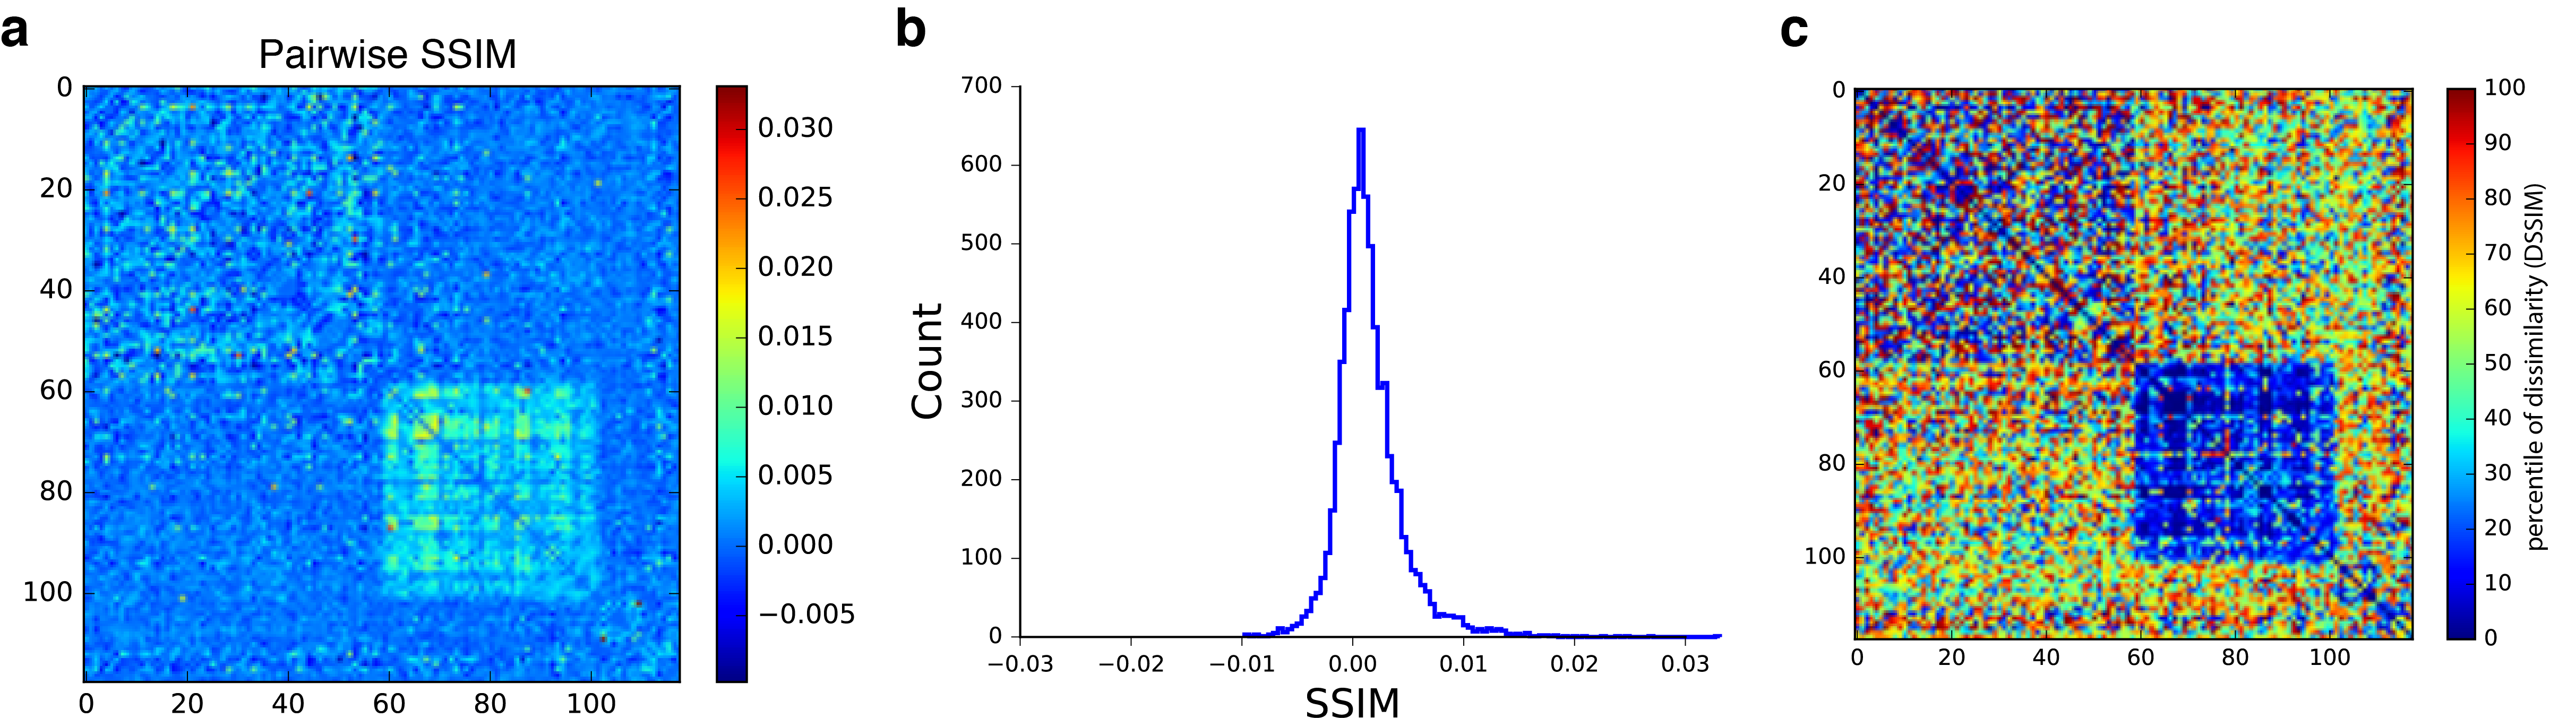
\includegraphics[scale=0.375]{Figures/chapter5/ssim_matrix_histogram_dssim.png}
%   \caption[Stimulus Set Image Similarity]{\textbf{Stimulus Set Image Similarity} }
%    \label{fig:SSIMhistDSSIM}
% \end{figure}
% %-----------------------------------------------------------------------------
% \begin{figure}
%   \centering
%    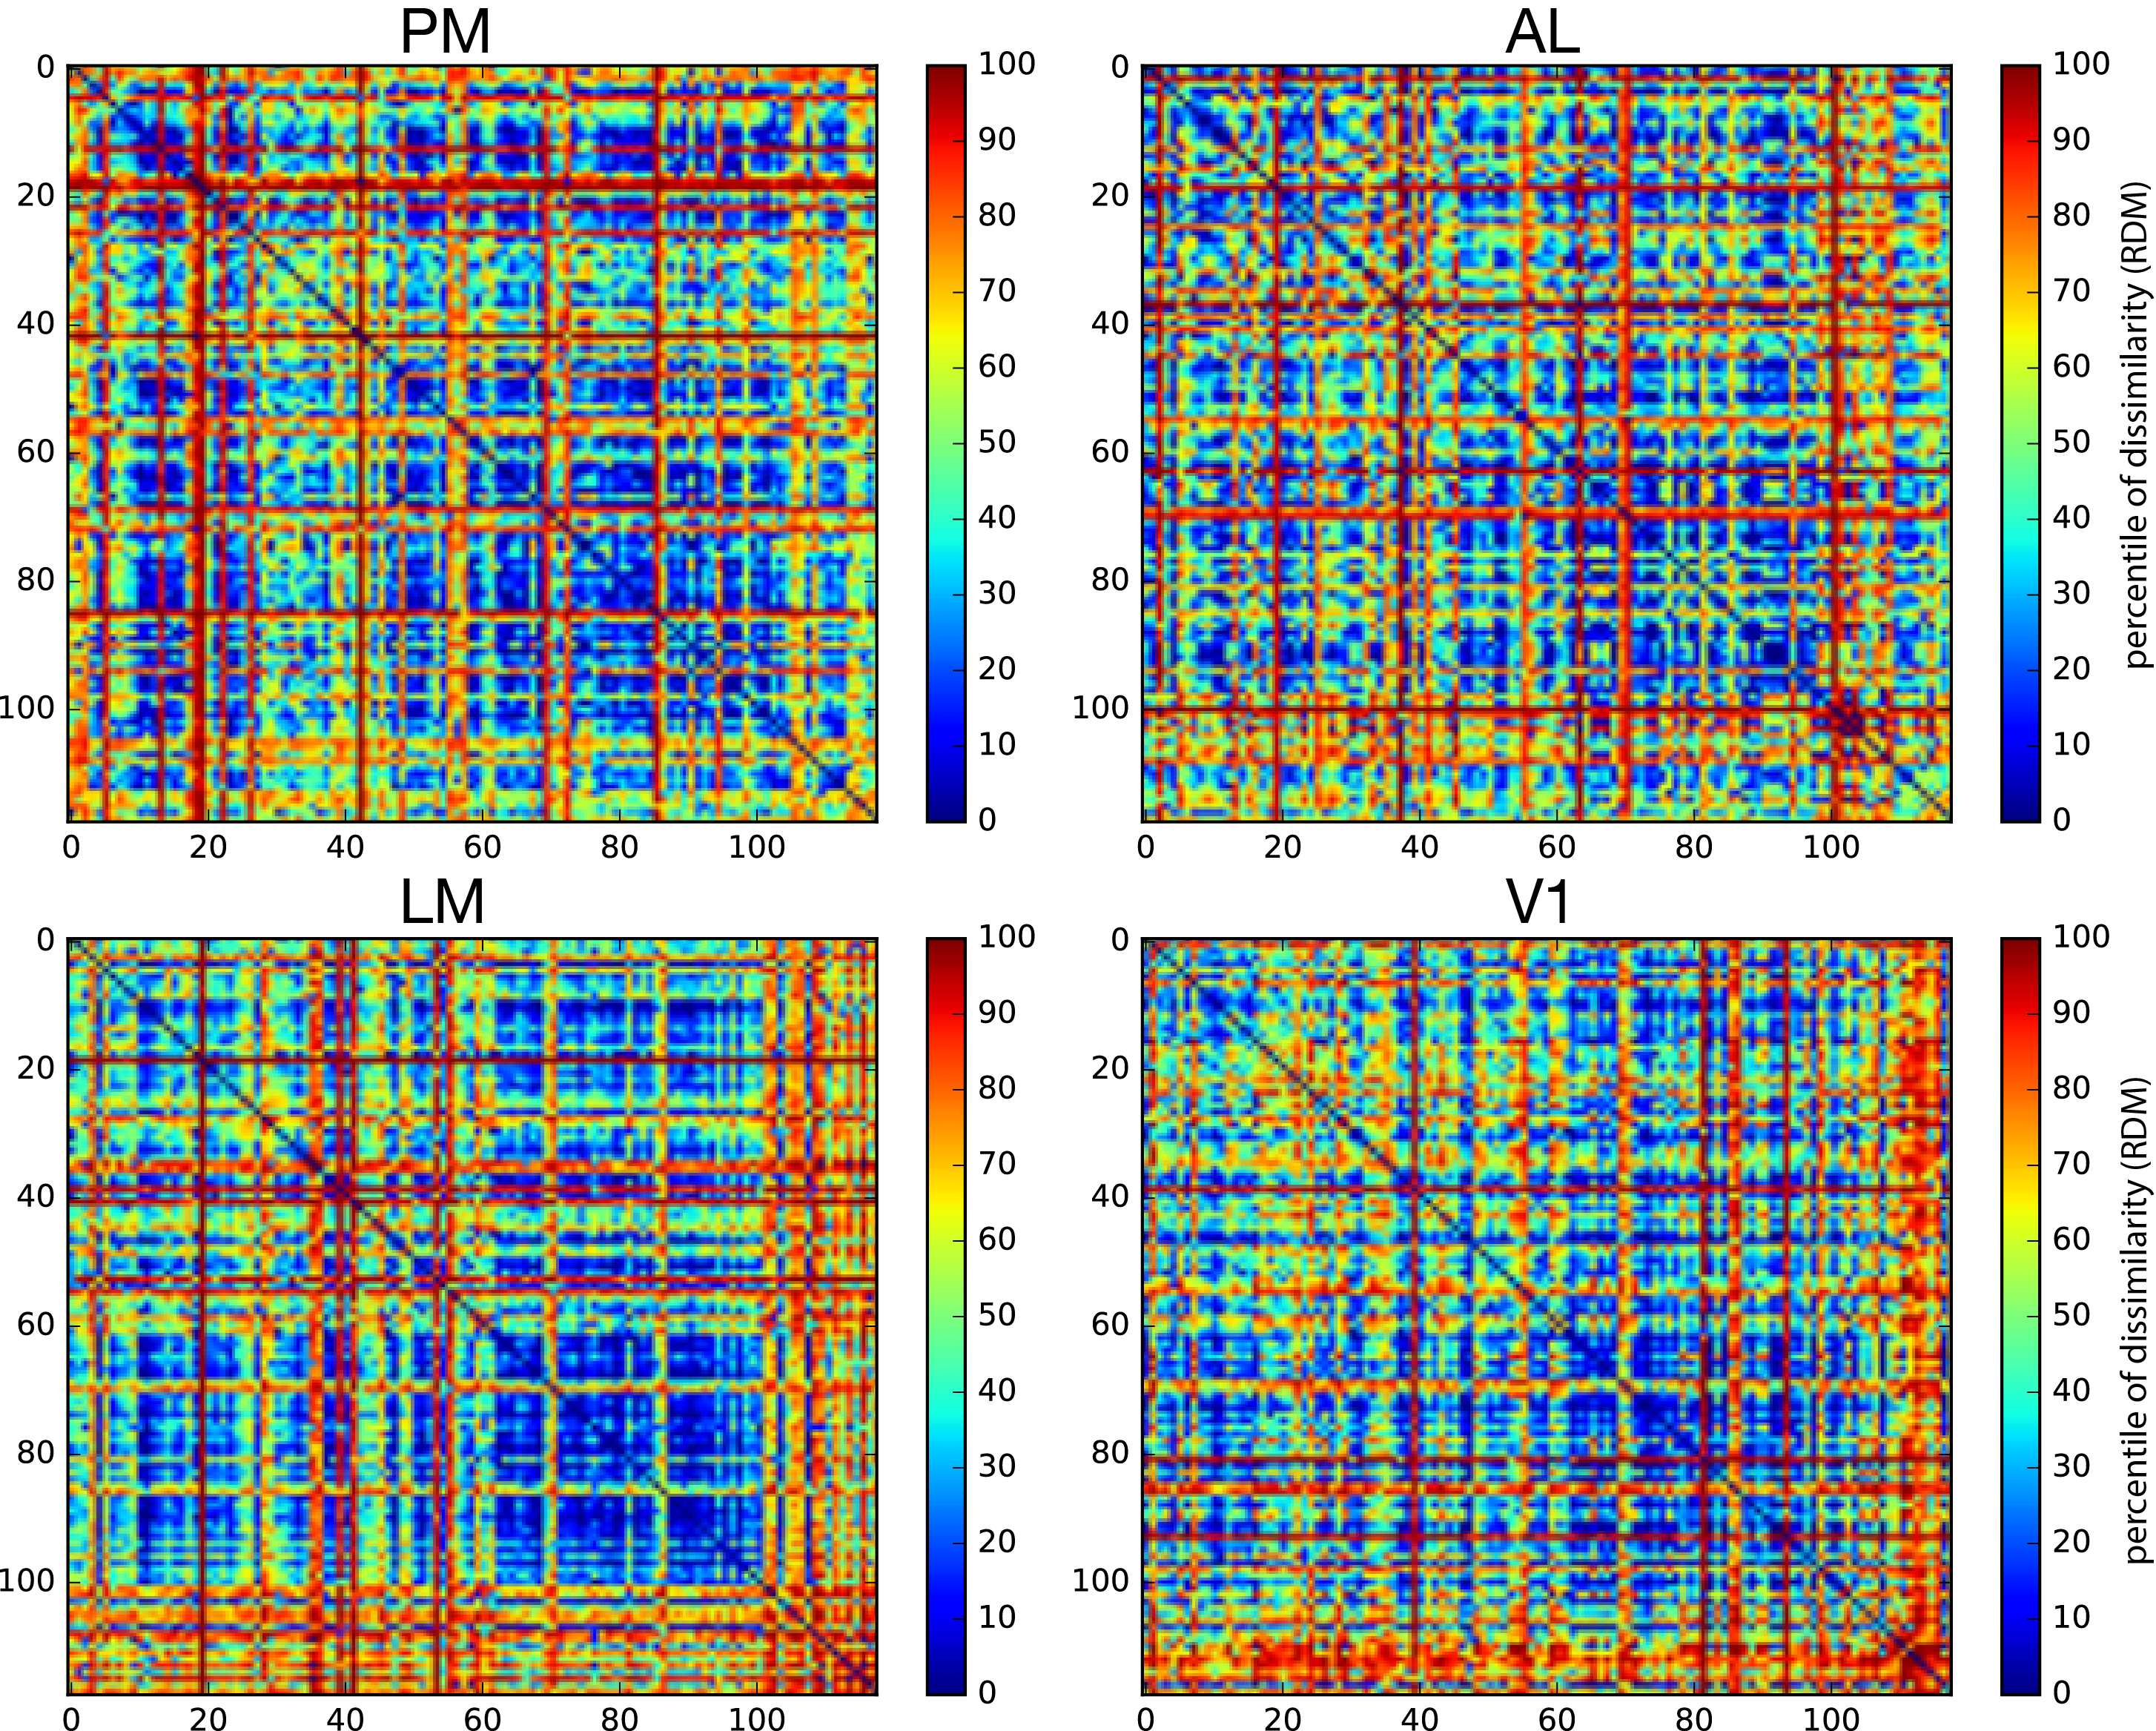
\includegraphics[width=\textwidth]{Figures/chapter5/rdm_percentiles.png}
%   \caption[Response Pattern Dissimilarity Matrices]{\textbf{Response Pattern Dissimilarity Matrices} Measured in percentile for  }
%    \label{fig:rdmper}
% \end{figure}
% %-----------------------------------------------------------------------------
% \begin{figure}
%   \centering
%    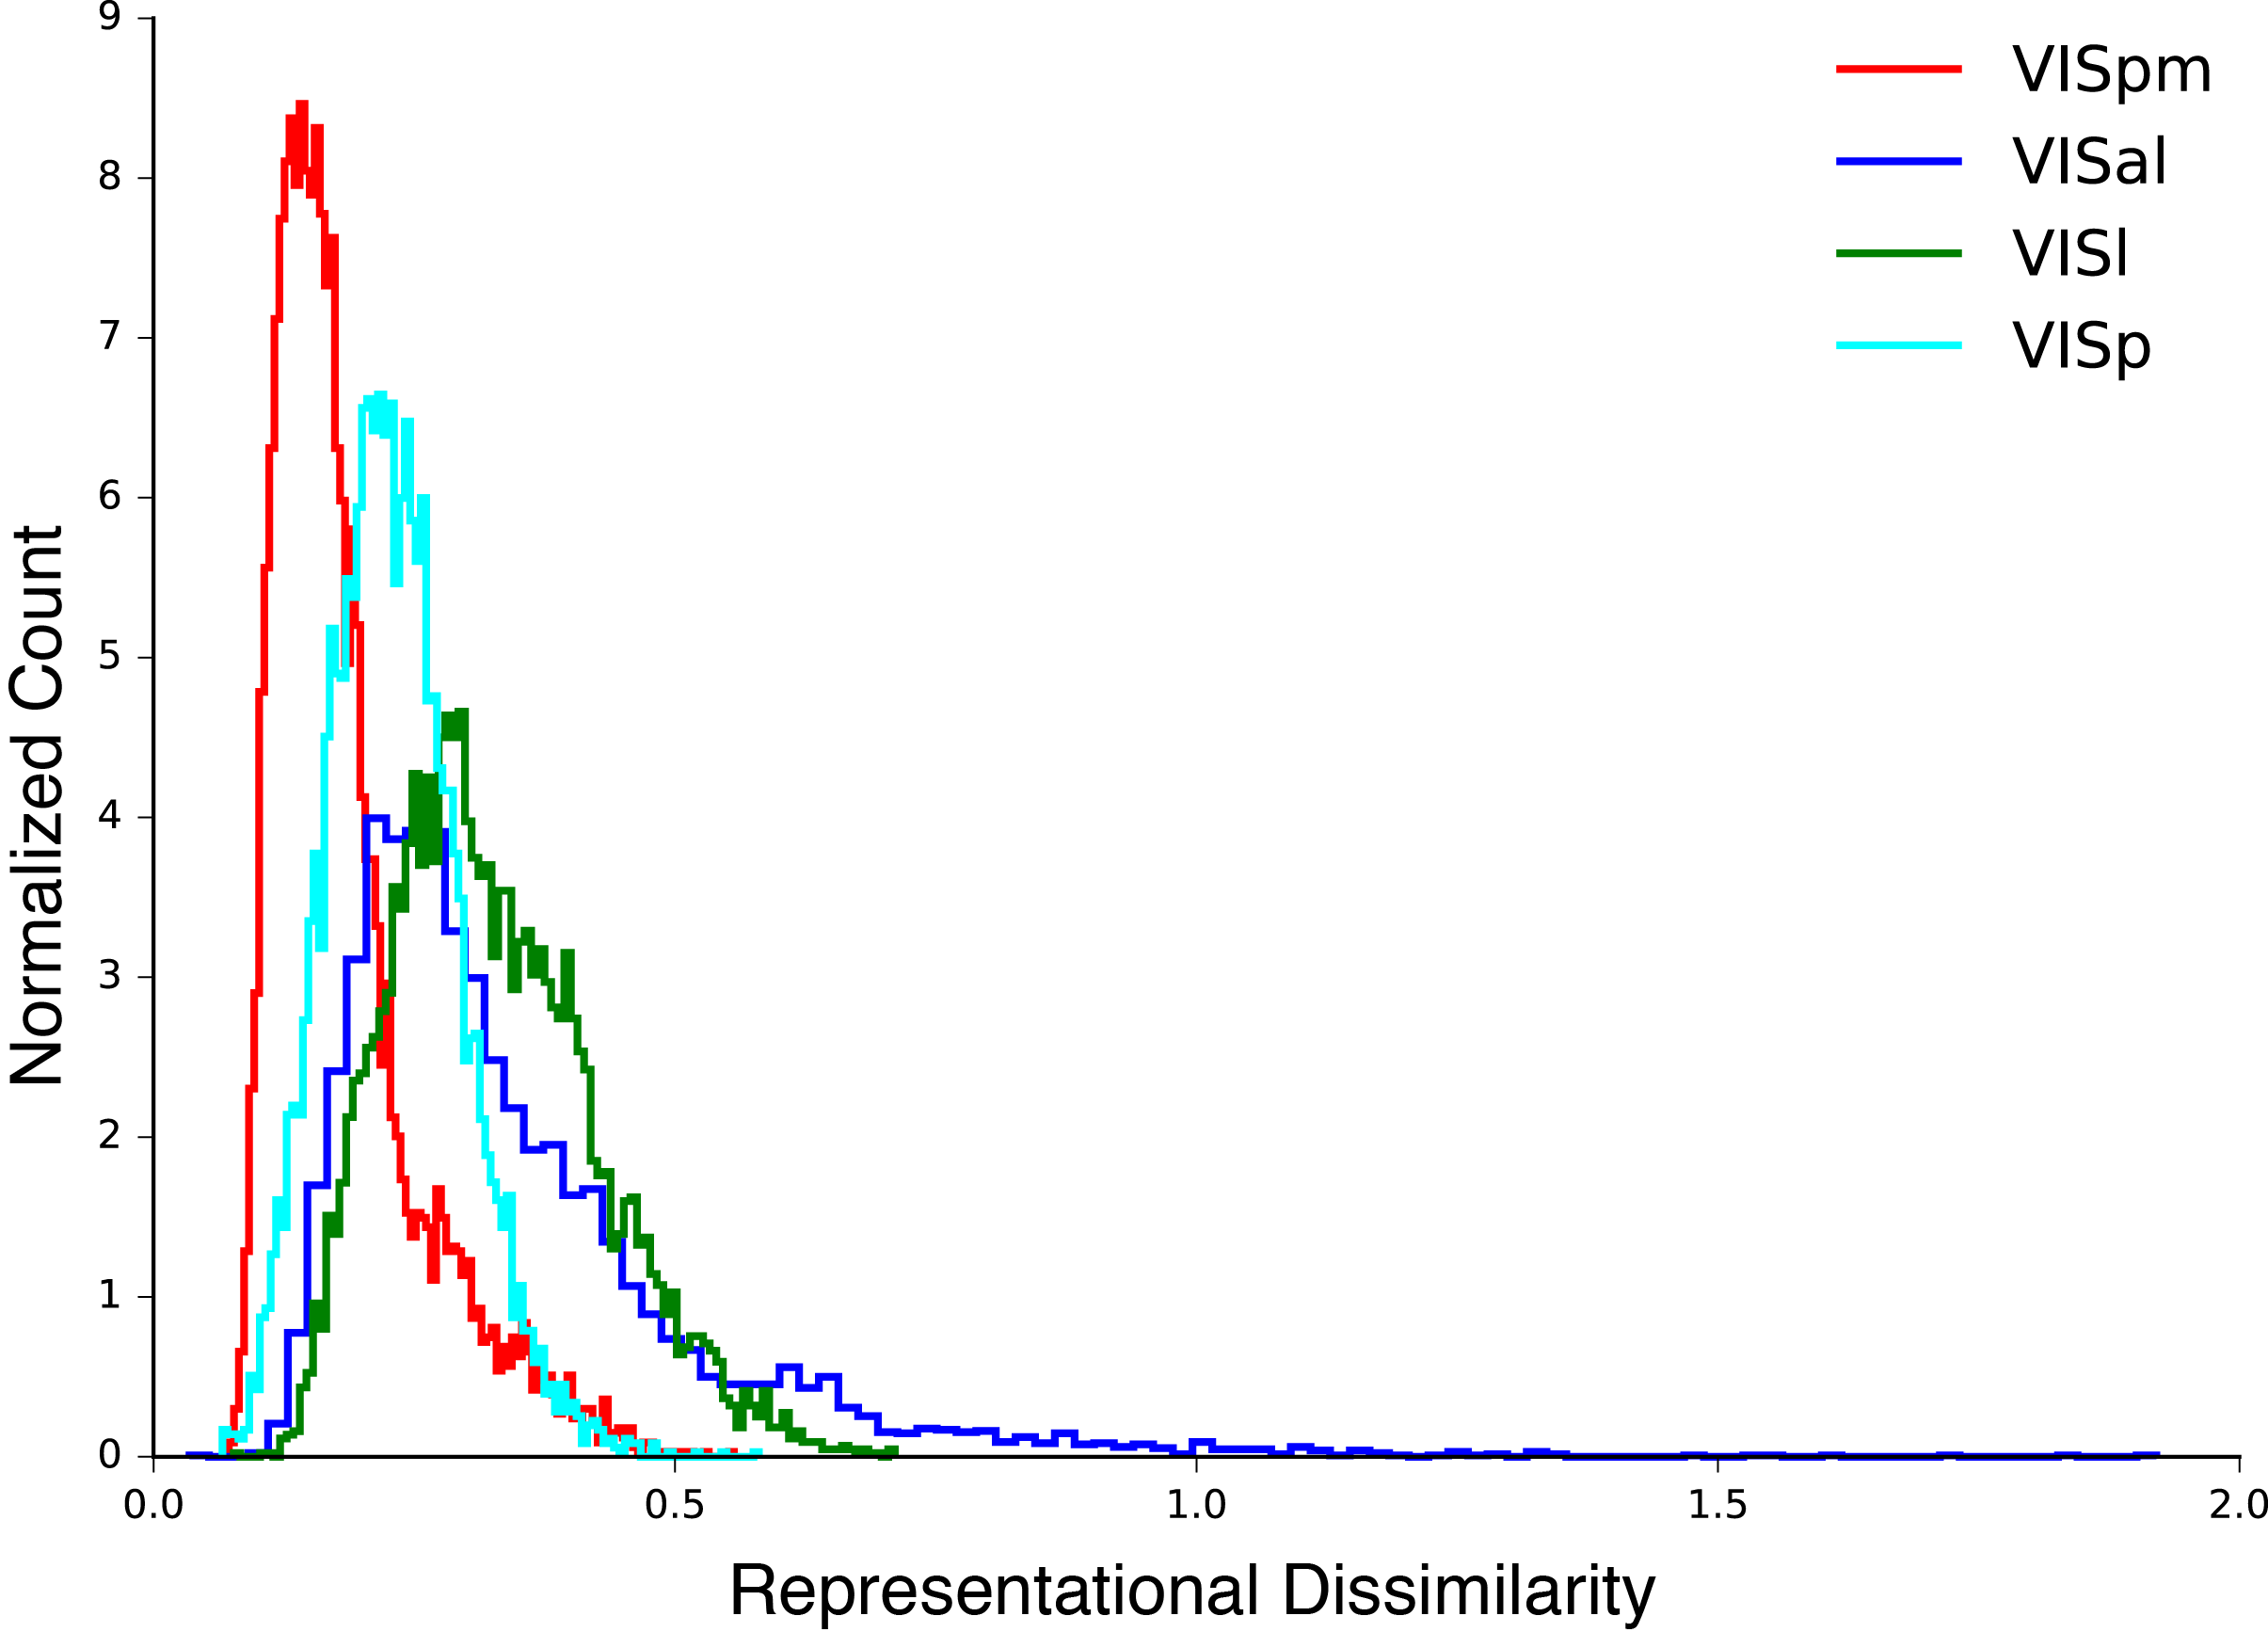
\includegraphics[scale=0.5]{Figures/chapter5/histogram_rdm.png}
%   \caption[]{\textbf{} }
%    \label{fig:histrdm}
% \end{figure}
% %-----------------------------------------------------------------------------

















